% Options for packages loaded elsewhere
% Options for packages loaded elsewhere
\PassOptionsToPackage{unicode}{hyperref}
\PassOptionsToPackage{hyphens}{url}
%
\documentclass[
  11pt,
  ignorenonframetext,
  aspectratio=169,
]{beamer}
\newif\ifbibliography
\usepackage{pgfpages}
\setbeamertemplate{caption}[numbered]
\setbeamertemplate{caption label separator}{: }
\setbeamercolor{caption name}{fg=normal text.fg}
\beamertemplatenavigationsymbolsempty
% remove section numbering
\setbeamertemplate{part page}{
  \centering
  \begin{beamercolorbox}[sep=16pt,center]{part title}
    \usebeamerfont{part title}\insertpart\par
  \end{beamercolorbox}
}
\setbeamertemplate{section page}{
  \centering
  \begin{beamercolorbox}[sep=12pt,center]{section title}
    \usebeamerfont{section title}\insertsection\par
  \end{beamercolorbox}
}
\setbeamertemplate{subsection page}{
  \centering
  \begin{beamercolorbox}[sep=8pt,center]{subsection title}
    \usebeamerfont{subsection title}\insertsubsection\par
  \end{beamercolorbox}
}
% Prevent slide breaks in the middle of a paragraph
\widowpenalties 1 10000
\raggedbottom
\AtBeginPart{
  \frame{\partpage}
}
\AtBeginSection{
  \ifbibliography
  \else
    \frame{\sectionpage}
  \fi
}
\AtBeginSubsection{
  \frame{\subsectionpage}
}
\usepackage{iftex}
\ifPDFTeX
  \usepackage[T1]{fontenc}
  \usepackage[utf8]{inputenc}
  \usepackage{textcomp} % provide euro and other symbols
\else % if luatex or xetex
  \usepackage{unicode-math} % this also loads fontspec
  \defaultfontfeatures{Scale=MatchLowercase}
  \defaultfontfeatures[\rmfamily]{Ligatures=TeX,Scale=1}
\fi
\usepackage{lmodern}

\ifPDFTeX\else
  % xetex/luatex font selection
\fi
% Use upquote if available, for straight quotes in verbatim environments
\IfFileExists{upquote.sty}{\usepackage{upquote}}{}
\IfFileExists{microtype.sty}{% use microtype if available
  \usepackage[]{microtype}
  \UseMicrotypeSet[protrusion]{basicmath} % disable protrusion for tt fonts
}{}
\makeatletter
\@ifundefined{KOMAClassName}{% if non-KOMA class
  \IfFileExists{parskip.sty}{%
    \usepackage{parskip}
  }{% else
    \setlength{\parindent}{0pt}
    \setlength{\parskip}{6pt plus 2pt minus 1pt}}
}{% if KOMA class
  \KOMAoptions{parskip=half}}
\makeatother

\usepackage{color}
\usepackage{fancyvrb}
\newcommand{\VerbBar}{|}
\newcommand{\VERB}{\Verb[commandchars=\\\{\}]}
\DefineVerbatimEnvironment{Highlighting}{Verbatim}{commandchars=\\\{\}}
% Add ',fontsize=\small' for more characters per line
\usepackage{framed}
\definecolor{shadecolor}{RGB}{241,243,245}
\newenvironment{Shaded}{\begin{snugshade}}{\end{snugshade}}
\newcommand{\AlertTok}[1]{\textcolor[rgb]{0.68,0.00,0.00}{#1}}
\newcommand{\AnnotationTok}[1]{\textcolor[rgb]{0.37,0.37,0.37}{#1}}
\newcommand{\AttributeTok}[1]{\textcolor[rgb]{0.40,0.45,0.13}{#1}}
\newcommand{\BaseNTok}[1]{\textcolor[rgb]{0.68,0.00,0.00}{#1}}
\newcommand{\BuiltInTok}[1]{\textcolor[rgb]{0.00,0.23,0.31}{#1}}
\newcommand{\CharTok}[1]{\textcolor[rgb]{0.13,0.47,0.30}{#1}}
\newcommand{\CommentTok}[1]{\textcolor[rgb]{0.37,0.37,0.37}{#1}}
\newcommand{\CommentVarTok}[1]{\textcolor[rgb]{0.37,0.37,0.37}{\textit{#1}}}
\newcommand{\ConstantTok}[1]{\textcolor[rgb]{0.56,0.35,0.01}{#1}}
\newcommand{\ControlFlowTok}[1]{\textcolor[rgb]{0.00,0.23,0.31}{\textbf{#1}}}
\newcommand{\DataTypeTok}[1]{\textcolor[rgb]{0.68,0.00,0.00}{#1}}
\newcommand{\DecValTok}[1]{\textcolor[rgb]{0.68,0.00,0.00}{#1}}
\newcommand{\DocumentationTok}[1]{\textcolor[rgb]{0.37,0.37,0.37}{\textit{#1}}}
\newcommand{\ErrorTok}[1]{\textcolor[rgb]{0.68,0.00,0.00}{#1}}
\newcommand{\ExtensionTok}[1]{\textcolor[rgb]{0.00,0.23,0.31}{#1}}
\newcommand{\FloatTok}[1]{\textcolor[rgb]{0.68,0.00,0.00}{#1}}
\newcommand{\FunctionTok}[1]{\textcolor[rgb]{0.28,0.35,0.67}{#1}}
\newcommand{\ImportTok}[1]{\textcolor[rgb]{0.00,0.46,0.62}{#1}}
\newcommand{\InformationTok}[1]{\textcolor[rgb]{0.37,0.37,0.37}{#1}}
\newcommand{\KeywordTok}[1]{\textcolor[rgb]{0.00,0.23,0.31}{\textbf{#1}}}
\newcommand{\NormalTok}[1]{\textcolor[rgb]{0.00,0.23,0.31}{#1}}
\newcommand{\OperatorTok}[1]{\textcolor[rgb]{0.37,0.37,0.37}{#1}}
\newcommand{\OtherTok}[1]{\textcolor[rgb]{0.00,0.23,0.31}{#1}}
\newcommand{\PreprocessorTok}[1]{\textcolor[rgb]{0.68,0.00,0.00}{#1}}
\newcommand{\RegionMarkerTok}[1]{\textcolor[rgb]{0.00,0.23,0.31}{#1}}
\newcommand{\SpecialCharTok}[1]{\textcolor[rgb]{0.37,0.37,0.37}{#1}}
\newcommand{\SpecialStringTok}[1]{\textcolor[rgb]{0.13,0.47,0.30}{#1}}
\newcommand{\StringTok}[1]{\textcolor[rgb]{0.13,0.47,0.30}{#1}}
\newcommand{\VariableTok}[1]{\textcolor[rgb]{0.07,0.07,0.07}{#1}}
\newcommand{\VerbatimStringTok}[1]{\textcolor[rgb]{0.13,0.47,0.30}{#1}}
\newcommand{\WarningTok}[1]{\textcolor[rgb]{0.37,0.37,0.37}{\textit{#1}}}

\usepackage{longtable,booktabs,array}
\newcounter{none} % for unnumbered tables
\usepackage{calc} % for calculating minipage widths
\usepackage{caption}
% Make caption package work with longtable
\makeatletter
\def\fnum@table{\tablename~\thetable}
\makeatother
\usepackage{graphicx}
\makeatletter
\newsavebox\pandoc@box
\newcommand*\pandocbounded[1]{% scales image to fit in text height/width
  \sbox\pandoc@box{#1}%
  \Gscale@div\@tempa{\textheight}{\dimexpr\ht\pandoc@box+\dp\pandoc@box\relax}%
  \Gscale@div\@tempb{\linewidth}{\wd\pandoc@box}%
  \ifdim\@tempb\p@<\@tempa\p@\let\@tempa\@tempb\fi% select the smaller of both
  \ifdim\@tempa\p@<\p@\scalebox{\@tempa}{\usebox\pandoc@box}%
  \else\usebox{\pandoc@box}%
  \fi%
}
% Set default figure placement to htbp
\def\fps@figure{htbp}
\makeatother





\setlength{\emergencystretch}{3em} % prevent overfull lines

\providecommand{\tightlist}{%
  \setlength{\itemsep}{0pt}\setlength{\parskip}{0pt}}



 


\setbeamertemplate{navigation symbols}{}
\setbeamertemplate{footline}[frame number]
\setbeamertemplate{itemize items}[circle]
\setbeamertemplate{itemize subitem}[triangle]
\setbeamercolor{frametitle}{fg=black}
\setbeamerfont{frametitle}{series=\bfseries}
\usepackage{amsmath}
\newcommand{\indep}{\perp\!\!\!\perp}
\usepackage{booktabs}
\usepackage{array}
\usepackage{adjustbox}
\usepackage{multirow}
\usepackage{dsfont}
\newcommand{\src}[1]{\par\vspace{-0.2em}{\tiny\color{gray} Source: #1}\par}
\usepackage{fancyvrb}
\fvset{fontsize=\scriptsize}
\makeatletter
\def\verbatim@font{\scriptsize\ttfamily}
\makeatother
\makeatletter
\@ifpackageloaded{caption}{}{\usepackage{caption}}
\AtBeginDocument{%
\ifdefined\contentsname
  \renewcommand*\contentsname{Table of contents}
\else
  \newcommand\contentsname{Table of contents}
\fi
\ifdefined\listfigurename
  \renewcommand*\listfigurename{List of Figures}
\else
  \newcommand\listfigurename{List of Figures}
\fi
\ifdefined\listtablename
  \renewcommand*\listtablename{List of Tables}
\else
  \newcommand\listtablename{List of Tables}
\fi
\ifdefined\figurename
  \renewcommand*\figurename{Figure}
\else
  \newcommand\figurename{Figure}
\fi
\ifdefined\tablename
  \renewcommand*\tablename{Table}
\else
  \newcommand\tablename{Table}
\fi
}
\@ifpackageloaded{float}{}{\usepackage{float}}
\floatstyle{ruled}
\@ifundefined{c@chapter}{\newfloat{codelisting}{h}{lop}}{\newfloat{codelisting}{h}{lop}[chapter]}
\floatname{codelisting}{Listing}
\newcommand*\listoflistings{\listof{codelisting}{List of Listings}}
\makeatother
\makeatletter
\makeatother
\makeatletter
\@ifpackageloaded{caption}{}{\usepackage{caption}}
\@ifpackageloaded{subcaption}{}{\usepackage{subcaption}}
\makeatother

\usepackage{bookmark}
\IfFileExists{xurl.sty}{\usepackage{xurl}}{} % add URL line breaks if available
\urlstyle{same}
\hypersetup{
  pdftitle={Difference-in-Differences: Composition{,} Triple Differences and Covariates},
  pdfauthor={Professor Ji-Woong Chung},
  hidelinks,
  pdfcreator={LaTeX via pandoc}}


\title{\texorpdfstring{Difference-in-Differences: Composition, Triple
Differences and
Covariates}{Difference-in-Differences: Composition{,} Triple Differences and Covariates}}
\subtitle{\texorpdfstring{BUSS975: Causal Inference in Financial
Research}{BUSS975: Causal Inference in Financial Research}}
\author{Professor Ji-Woong Chung}
\date{}
\institute{Korea University}

\begin{document}
\frame{\titlepage}


\begin{frame}{Where we left off}
\protect\phantomsection\label{where-we-left-off}
\begin{itemize}
\tightlist
\item
  Lecture 7: difference-in-differences is \textbf{four averages and
  three subtractions}.
\item
  It identifies the ATT if the two groups' untreated outcomes would have
  moved in parallel, and the baseline is untreated.
\end{itemize}

\vspace{0.5em}

\begin{itemize}
\tightlist
\item
  Considered \textbf{one} treated group, \textbf{one} control group and
  \textbf{one} date.
\item
  This lecture and the next ask what happens when the design stops being
  a single \(2 \times 2\).
\end{itemize}
\end{frame}

\begin{frame}{Four ways the single \(2 \times 2\) breaks}
\protect\phantomsection\label{four-ways-the-single-2-times-2-breaks}
\begin{enumerate}
\tightlist
\item
  \textbf{The sample changes under your feet.} Units drop out; a
  repeated cross-section draws different people.
\item
  \textbf{The trends are not parallel}, but a second comparison inside
  the same states might share the bias. \emph{Triple differences.}
\item
  \textbf{The groups differ in ways you can measure.} Parallel trends
  holds only among similar units. \emph{Covariates.}
\item
  \textbf{Treatment arrives at different dates.} TWFE quietly becomes a
  weighted average of comparisons nobody chose.
\end{enumerate}
\end{frame}

\section{1. Who Is in the Sample}\label{who-is-in-the-sample}

\begin{frame}{Imbalanced panels: is missing data a problem?}
\protect\phantomsection\label{imbalanced-panels-is-missing-data-a-problem}
\begin{itemize}
\tightlist
\item
  A panel follows the same units. When some drop out or reappear, the
  panel is \textbf{imbalanced}.
\item
  Parallel trends is a statement about the \textbf{average change} in
  \(Y^0\). Missing units matter only if they change that average.
\item
  If units go missing \textbf{at random}, the average is unaffected.
\item
  Weaker and enough: missingness \(M\) is unrelated to the
  \emph{untreated} outcome, given covariates, \[
  Y^0 \;\indep\; M \mid X \qquad\Longrightarrow\qquad \mathbb{E}[Y^0 \mid M=1, X] = \mathbb{E}[Y^0 \mid M=0, X].
  \]
\end{itemize}
\end{frame}

\begin{frame}{Two people who leave}
\protect\phantomsection\label{two-people-who-leave}
\begin{itemize}
\tightlist
\item
  \textbf{Maria} (treated) leaves because the training got her promoted.

  \begin{itemize}
  \tightlist
  \item
    She is missing because of her \(Y^1\), not her \(Y^0\).
  \item
    The untreated trend is untouched. Her absence changes \emph{which}
    treated outcomes we see, not the counterfactual.
  \end{itemize}
\item
  \textbf{Inez} (control) drops out in year 4, for reasons unrelated to
  \(Y^0\) given \(X\).

  \begin{itemize}
  \tightlist
  \item
    Impute her missing \emph{observed} outcome from untreated units like
    her.
  \item
    A missing-data problem, not an identification problem.
  \end{itemize}
\end{itemize}

\vspace{0.4em}

\begin{itemize}
\tightlist
\item
  The rule: know \textbf{why} units are missing before you drop them.
\end{itemize}
\end{frame}

\begin{frame}{Repeated cross-sections: did Napster kill music sales?}
\protect\phantomsection\label{repeated-cross-sections-did-napster-kill-music-sales}
\begin{center}
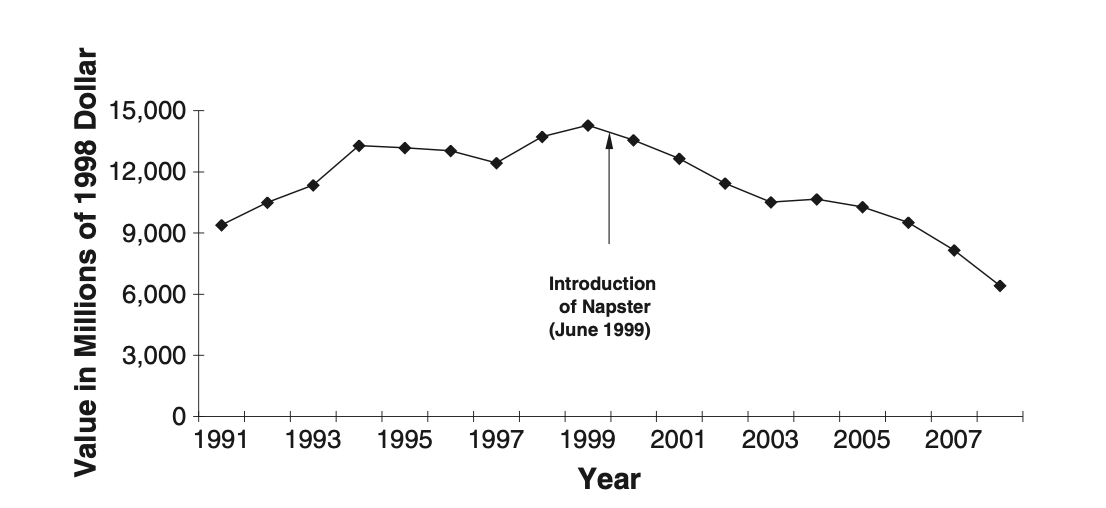
\includegraphics[height=4.3cm]{figs/remix10-01.png}
\end{center}
\src{Hong (2013), reproduced in Cunningham (2025), Figure 10.1.}

\begin{itemize}
\tightlist
\item
  Record sales peak in 1999, the year Napster arrived. Coincidence, or
  cause?
\item
  Hong (2013) compares \textbf{internet users} with \textbf{non-users}
  in the Consumer Expenditure Survey: a fresh random sample every year.
\end{itemize}
\end{frame}

\begin{frame}{Who is ``treated'' changes over time}
\protect\phantomsection\label{who-is-treated-changes-over-time}
\begin{center}\small
\begin{tabular}{lcccccccc}
\toprule
 & \multicolumn{2}{c}{1997} & \multicolumn{2}{c}{1998} & \multicolumn{2}{c}{1999} & \multicolumn{2}{c}{2000} \\
 & User & Non & User & Non & User & Non & User & Non \\
\midrule
Age & 40.2 & 49.0 & 42.3 & 49.0 & 44.1 & 49.4 & 44.3 & 49.9 \\
Income (\$000) & 52.9 & 30.5 & 52.0 & 26.2 & 50.0 & 26.6 & 47.5 & 26.3 \\
College graduate & 0.43 & 0.21 & 0.45 & 0.21 & 0.42 & 0.20 & 0.37 & 0.20 \\
\bottomrule
\end{tabular}
\end{center}

\begin{itemize}
\tightlist
\item
  As internet use spread, the ``treated'' group got \textbf{older,
  poorer and less educated}.
\item
  Older people buy less music. So users' spending falls even if Napster
  does nothing.
\item
  Parallel trends breaks \textbf{because different people are sampled.}
\end{itemize}
\end{frame}

\begin{frame}{Diagnosing compositional change}
\protect\phantomsection\label{diagnosing-compositional-change}
\begin{itemize}
\tightlist
\item
  \textbf{Diagnostic 1.} A balance table \emph{over time}, like the
  previous one, not just at baseline.
\item
  \textbf{Diagnostic 2.} Run the DiD with an exogenous covariate as the
  \emph{outcome}: \[
  X_{it} = \alpha + \beta_1 D_i + \beta_2 \text{Post}_t + \delta\,(D_i \times \text{Post}_t) + \varepsilon_{it}.
  \]
\item
  Napster cannot make anyone older. A significant \(\hat\delta\) says
  the sample's composition shifted at treatment.
\item
  If that \(X\) also predicts \(Y^0\), parallel trends is mechanically
  broken.
\end{itemize}
\end{frame}

\begin{frame}{Repairing it: reweight each period (Hong 2013)}
\protect\phantomsection\label{repairing-it-reweight-each-period-hong-2013}
\begin{enumerate}
\tightlist
\item
  Estimate \textbf{two} propensity scores, one per period:
  \(P_b = \Pr(D=1 \mid T=0, X)\) and \(P_a = \Pr(D=1 \mid T=1, X)\).
\item
  Compute the four group-period means with inverse-probability weights
  from \textbf{their own period's} score.
\item
  Take the \(2 \times 2\) of the weighted means. Equivalently, the usual
  DiD regression by weighted least squares.
\end{enumerate}

\vspace{0.4em}

\begin{itemize}
\tightlist
\item
  Intuition: reweight every year's sample to have the \textbf{same mix
  of \(X\)}. Then each group's mix of X is the same in every year, so
  composition cannot move the DiD.
\item
  Panels are expensive; much of the world's data are repeated
  cross-sections. See also Sant'Anna and Xu (2023).
\end{itemize}
\end{frame}

\section{2. Triple Differences}\label{triple-differences}

\begin{frame}{Gruber (1994): who pays for maternity benefits?}
\protect\phantomsection\label{gruber-1994-who-pays-for-maternity-benefits}
\begin{itemize}
\tightlist
\item
  Some states mandated that employer health insurance cover maternity.
\item
  The mandate makes insuring women of childbearing age costlier. Who
  pays?
\item
  If employers can cut these women's wages, the women pay. If they
  cannot, employers hire fewer of them. Gruber asks: do their wages
  fall?
\item
  The obvious DiD: married women aged 20--40, mandate states vs.~other
  states, before vs.~after. Writing \(NJ\) for mandate states and \(PA\)
  for the rest, \[
  \hat\delta = \underbrace{D}_{\text{effect}} + \underbrace{(NJ_t - PA_t)}_{\text{non-parallel trends bias}} .
  \]
\item
  Gruber worried that state labour markets were on different paths for
  reasons unrelated to the mandate. Then this DiD is biased.
\end{itemize}
\end{frame}

\begin{frame}{The fix: a second DiD in the same states}
\protect\phantomsection\label{the-fix-a-second-did-in-the-same-states}
\begin{itemize}
\tightlist
\item
  Find a group in the \textbf{same states} that the law does not touch:
  single men aged 20--40 and workers over 40.
\item
  Their DiD has no effect in it, only the bias:
  \(\hat\delta_{\text{alt}} = (NJ_t - PA_t)\).
\item
  Subtract: \[
  \hat\delta_{DDD} = \hat\delta_{\text{primary}} - \hat\delta_{\text{alt}} = D + (NJ_t - PA_t) - (NJ_t - PA_t) = D.
  \]
\item
  Intuition: the second DiD \textbf{measures the bias} of the first.
  Whatever made mandate states' labour markets drift, it shows up for
  the untouched workers too.
\end{itemize}
\end{frame}

\begin{frame}{Two biased DiDs, one unbiased triple difference}
\protect\phantomsection\label{two-biased-dids-one-unbiased-triple-difference}
\begin{center}
\includegraphics[width=0.84\linewidth,height=\textheight,keepaspectratio]{08a_did_covariates_files/figure-beamer/ddd-sim-1.pdf}
\end{center}

\src{Simulated, after Cunningham (2025), Figure 10.3: both groups share a bias of $-500$ a year; true effect $-5{,}000$.}

\begin{itemize}
\tightlist
\item
  Both DiDs show the same falling pre-trend. Their difference (green) is
  flat before and \(-5{,}000\) after.
\end{itemize}
\end{frame}

\begin{frame}{The assumption: parallel bias}
\protect\phantomsection\label{the-assumption-parallel-bias}
\begin{itemize}
\tightlist
\item
  With \(D\) the state and \(G\) the eligible group, DDD needs the
  \textbf{same bias} for both groups (Olden and Møen 2022): \[
  \begin{aligned}
  &\mathbb{E}[\Delta Y^0 \mid D=1, G=1] - \mathbb{E}[\Delta Y^0 \mid D=0, G=1] \\
  &\qquad = \mathbb{E}[\Delta Y^0 \mid D=1, G=0] - \mathbb{E}[\Delta Y^0 \mid D=0, G=0].
  \end{aligned}
  \]
\item
  The second DiD is \textbf{not required to be zero}, only equal to the
  first DiD's bias.
\item
  If it \emph{were} zero, the first DiD was fine all along. The second
  group would then be a falsification (``same outcome, different
  group''), as with Miller, Johnson and Wherry's elderly in Lecture 7.
\item
  So triple differences is a \textbf{design}, not a falsification.
\end{itemize}
\end{frame}

\begin{frame}{Triple differences by regression}
\protect\phantomsection\label{triple-differences-by-regression}
Eight averages and seven subtractions. Identical to OLS with
\textbf{all} interactions of period \(\text{Post}_t\), group \(G_g\) and
state \(D_i\): \[
\begin{aligned}
Y_{igt} = \alpha &+ \beta_1 \text{Post}_t + \beta_2 G_g + \beta_3 D_i + \beta_4 (G_g \cdot \text{Post}_t) \\
&+ \beta_5 (D_i \cdot \text{Post}_t) + \beta_6 (D_i \cdot G_g) + \beta_7 (D_i \cdot G_g \cdot \text{Post}_t) + \varepsilon_{igt}.
\end{aligned}
\]

\begin{itemize}
\tightlist
\item
  \(\beta_7\) is the triple difference. Drop any of the two-way terms
  and it no longer is.
\item
  Event study: replace \(\text{Post}_t\) with a dummy for every period
  except the last one before treatment.
\end{itemize}

\vspace{0.3em}

In practice:

\begin{itemize}
\tightlist
\item
  \textbf{Cluster} where the law varies: the state.
\item
  \textbf{Show three event studies}: each DiD, and their difference. The
  two DiDs' pre-trends should look alike; that is the visible part of
  ``parallel bias''.
\end{itemize}
\end{frame}

\begin{frame}{Gruber's result}
\protect\phantomsection\label{grubers-result}
\begin{center}\scriptsize
\begin{tabular}{lccc}
\toprule
Log hourly wage & Before & After & Difference \\
\midrule
\multicolumn{4}{l}{\emph{A. Married women 20--40}} \\
Experimental states & 1.547 & 1.513 & $-0.034$ \\
Non-experimental states & 1.369 & 1.397 & $0.028$ \\
Difference-in-differences & & & $\mathbf{-0.062}$ (0.022) \\
\midrule
\multicolumn{4}{l}{\emph{B. Over 40 and single men 20--40}} \\
Experimental states & 1.759 & 1.748 & $-0.011$ \\
Non-experimental states & 1.630 & 1.627 & $-0.003$ \\
Difference-in-differences & & & $\mathbf{-0.008}$ (0.014) \\
\midrule
Triple difference & & & $\mathbf{-0.054}$ (0.026) \\
\bottomrule
\end{tabular}
\end{center}

\begin{itemize}
\tightlist
\item
  Panel B \emph{estimates the bias} of panel A. It is small, so DDD and
  DiD nearly agree.
\item
  Married women's wages fell about \(5\) percent: the mandate was paid
  for by the workers it protected.
\end{itemize}
\end{frame}

\section{3. Covariates}\label{covariates}

\begin{frame}{Covariates: the plan}
\protect\phantomsection\label{covariates-the-plan}
\begin{itemize}
\tightlist
\item
  Parallel trends that holds only among units that \textbf{look alike}.
\item
  It is the most common reason researchers add controls to a DiD
  regression.
\end{itemize}

\vspace{0.4em}

\begin{itemize}
\tightlist
\item
  \textbf{3.1 Why covariates enter}, and which ones.
\item
  \textbf{3.2 A running example} in which parallel trends fails but
  conditional parallel trends holds.
\item
  \textbf{3.3 What the usual regressions do with it}: two ways TWFE goes
  wrong, and the fixes.
\item
  \textbf{3.4 IPW, outcome regression, doubly robust}: each recovers the
  ATT in the example.
\item
  \textbf{3.5 Simulation}
\end{itemize}
\end{frame}

\begin{frame}{Levels, trends, and why covariates enter}
\protect\phantomsection\label{levels-trends-and-why-covariates-enter}
\begin{itemize}
\tightlist
\item
  Parallel trends is about trends, not levels. Groups at different
  levels are fine \textbf{in principle}.
\item
  In practice a large level gap is a warning: whatever made the groups
  different might also make their untreated \emph{trends} different.
\item
  Kahn-Lang and Lang (2020): every DiD paper should say why the levels
  differ and why that would not affect the trends.
\item
  The \textbf{distribution of covariates} can cause both a level gap and
  different untreated trends (\(\Delta \mathbb{E}[Y^0]\)). Then
  condition on them, \textbf{conditional parallel trends} (Heckman et
  al.~1997): \[
  \mathbb{E}[Y^0_{\text{post}} - Y^0_{\text{pre}} \mid D=1, X] \;=\; \mathbb{E}[Y^0_{\text{post}} - Y^0_{\text{pre}} \mid D=0, X].
  \]
\end{itemize}
\end{frame}

\begin{frame}{What conditioning buys, and what it costs}
\protect\phantomsection\label{what-conditioning-buys-and-what-it-costs}
\begin{itemize}
\tightlist
\item
  \textbf{Buys}: parallel trends only among units with the \textbf{same
  \(X\)}. Young treated workers are compared with young controls, old
  with old.
\item
  \textbf{Costs} two things:

  \begin{itemize}
  \tightlist
  \item
    \textbf{common support}: for every treated \(X\) there must be
    controls with that \(X\), or a functional form that extrapolates
    where there are none;
  \item
    a decision about \textbf{which} \(X\).
  \end{itemize}
\end{itemize}

\vspace{0.4em}

\begin{itemize}
\tightlist
\item
  Example: if young workers' earnings grow faster and the treated are
  mostly young, the raw DiD mixes the treatment effect with an
  age-driven trend. Conditioning on age removes the age-driven part.
\end{itemize}
\end{frame}

\begin{frame}{Which covariates?}
\protect\phantomsection\label{which-covariates}
\begin{center}
\includegraphics[width=0.4\linewidth,height=\textheight,keepaspectratio]{08a_did_covariates_files/figure-beamer/dag-x-1.pdf}
\end{center}

\(X\) must do \textbf{both} things:

\begin{enumerate}
\tightlist
\item
  \(X \rightarrow D\): it is distributed differently in treated and
  control groups;
\item
  \(X \rightarrow \Delta \mathbb{E}[Y^0]\): it drives the untreated
  \textbf{trend}.
\end{enumerate}

\begin{itemize}
\tightlist
\item
  Only the first: harmless but useless. Only the second: precision, not
  identification.
\item
  But both: a confounder of trends.
\end{itemize}
\end{frame}

\begin{frame}{Measure \(X\) at baseline}
\protect\phantomsection\label{measure-x-at-baseline}
\begin{itemize}
\tightlist
\item
  \textbf{Never} a covariate that \textbf{responds to treatment} (a bad
  control). A value measured after treatment is safe only if treatment
  cannot move it; the baseline value is safe by construction.
\item
  The list can swing the estimate a lot. Fix it before you see results,
  and say so.
\end{itemize}

\vspace{0.4em}

\begin{itemize}
\tightlist
\item
  \textbf{Convention for the rest of Section 3:} each unit's \(X\) is
  measured \textbf{once, before treatment}, and held fixed. We write
  \(X_i\), never \(X_{it}\). Age changes; we use age at baseline.
\item
  \emph{The Remix} writes its derivation with a time-varying \(X_{it}\).
  What changes then is in the Backup (``Time-varying \(X\)'').
\end{itemize}
\end{frame}

\begin{frame}{Is there imbalance? The LaLonde data}
\protect\phantomsection\label{is-there-imbalance-the-lalonde-data}
The standardized mean difference from Lecture 3b, on the job-training
data:

\begin{center}\small
\begin{tabular}{lccc}
\toprule
 & Mean treated & Mean control & SMD \\
\midrule
Age & 25.8 & 33.2 & $-0.80$ \\
Education & 10.3 & 12.0 & $-0.68$ \\
Black & 0.84 & 0.07 & $2.43$ \\
Hispanic & 0.06 & 0.07 & $-0.05$ \\
Married & 0.19 & 0.71 & $-1.23$ \\
Unemployed 1974 & 0.71 & 0.12 & $1.49$ \\
\bottomrule
\end{tabular}
\end{center}

\begin{itemize}
\tightlist
\item
  Everything but Hispanic is far past Lecture 3b's line of \(0.1\), and
  past the looser \(0.25\) of Imbens and Rubin (2015).
\item
  Irrelevant if these variables do not drive earnings \emph{trends};
  fatal if they do. Either way, use conditional parallel trends and an
  estimator built for it.
\end{itemize}
\end{frame}

\begin{frame}{Four ways to use conditional parallel trends}
\protect\phantomsection\label{four-ways-to-use-conditional-parallel-trends}
\begin{center}\small
\begin{tabular}{lll}
\toprule
Estimator & What it does & What must be right \\
\midrule
TWFE $+\,\theta X$ & adds $X$ linearly to the regression & no $X$-specific trends; with \\
 & & $X \cdot \text{Post}$, homogeneous effects \\
IPW (Abadie 2005) & reweights controls to look like the treated & the propensity score \\
Outcome regression & predicts the treated's $\Delta Y^0$ from controls & the outcome model \\
Doubly robust & both at once & either one of the two \\
\bottomrule
\end{tabular}
\end{center}

\begin{itemize}
\tightlist
\item
  All four target the same thing: the \textbf{counterfactual change} of
  the treated, built from controls with the same \(X\).
\end{itemize}
\end{frame}

\section{3.2 A Running Example}\label{a-running-example}

\begin{frame}{Young and old: the setup}
\protect\phantomsection\label{young-and-old-the-setup}
\(200\) units, two periods. \(X\) is young or old, fixed at baseline.
Most treated units are young.

\begin{center}\small
\begin{tabular}{lcccccc}
\toprule
 & \# units & $\Pr(\text{young})$ & $Y^0_{\text{pre}}$ & $Y^0_{\text{post}}$ & $\Delta Y^0$ & Group average $\Delta Y^0$ \\
\midrule
Treated, old & 20 & \multirow{2}{*}{$\bar X_1 = 0.8$} & 34 & \textbf{36} & 2 & \multirow{2}{*}{$0.8 \times 10 + 0.2 \times 2 = 8.4$} \\
Treated, young & 80 & & 24 & \textbf{34} & 10 & \\
\addlinespace
Control, old & 80 & \multirow{2}{*}{$\bar X_0 = 0.2$} & 30 & 32 & 2 & \multirow{2}{*}{$0.2 \times 10 + 0.8 \times 2 = 3.6$} \\
Control, young & 20 & & 20 & 30 & 10 & \\
\bottomrule
\end{tabular}
\end{center}

\begin{itemize}
\tightlist
\item
  The treated start \(4\) higher at every age: a \textbf{level} gap,
  which DiD allows.
\item
  Young units' untreated outcome grows by \(10\), old units' by \(2\),
  \textbf{in both groups}. Conditional parallel trends holds by
  construction. The group averages differ, \(8.4\) against \(3.6\).
\item
  The treated's \(Y^0_{\text{post}}\) is never observed.
\end{itemize}
\end{frame}

\begin{frame}{Parallel trends fails; conditional parallel trends holds}
\protect\phantomsection\label{parallel-trends-fails-conditional-parallel-trends-holds}
\begin{center}
\includegraphics[width=0.92\linewidth,height=\textheight,keepaspectratio]{08a_did_covariates_files/figure-beamer/ex-fig-1.pdf}
\end{center}

\begin{itemize}
\tightlist
\item
  Within each age the trends are parallel. The gap comes from
  \textbf{who} is in each group: the treated are mostly young, and the
  young grow faster.
\end{itemize}
\end{frame}

\begin{frame}{The truth: two scenarios, one ATT}
\protect\phantomsection\label{the-truth-two-scenarios-one-att}
\(\Delta Y = Y_{\text{post}} - Y_{\text{pre}}\) is the \textbf{observed}
change. For a treated unit, \(Y_{\text{pre}} = Y^0_{\text{pre}}\) (no
anticipation) and
\(Y_{\text{post}} = Y^0_{\text{post}} + \text{effect}\), so
\(\Delta Y = \Delta Y^0 + \text{effect}.\)

\begin{center}\small
\begin{tabular}{lcccccc}
\toprule
 & & & \multicolumn{2}{c}{Homogeneous} & \multicolumn{2}{c}{Heterogeneous} \\
\cmidrule(lr){4-5} \cmidrule(lr){6-7}
 & \# units & $\Delta Y^0$ & Effect & $\Delta Y$ & Effect & $\Delta Y$ \\
\midrule
Treated, old & 20 & 2 & 5 & 7 & 1 & 3 \\
Treated, young & 80 & 10 & 5 & 15 & 6 & 16 \\
\addlinespace
Control, old & 80 & 2 & 0 & 2 & 0 & 2 \\
Control, young & 20 & 10 & 0 & 10 & 0 & 10 \\
\midrule
ATT & & & \multicolumn{2}{c}{$0.8 \times 5 + 0.2 \times 5 = 5$} & \multicolumn{2}{c}{$0.8 \times 6 + 0.2 \times 1 = 5$} \\
\bottomrule
\end{tabular}
\end{center}

\begin{itemize}
\tightlist
\item
  The ATT weights each age by its share \textbf{of the treated}, \(0.8\)
  and \(0.2\).
\item
  The treated's average change is
  \(0.2 \times 7 + 0.8 \times 15 = 0.2 \times 3 + 0.8 \times 16 = 13.4\).
\end{itemize}
\end{frame}

\begin{frame}{The raw DiD: 9.8}
\protect\phantomsection\label{the-raw-did-9.8}
\[
\hat\delta^{DD} = \underbrace{13.4}_{\text{treated } \Delta Y} - \underbrace{3.6}_{\text{control } \Delta Y} = 9.8, \qquad \text{vs. ATT} = 5 .
\] The bias is the gap in untreated trends, and it factors into two
pieces: \[
\underbrace{8.4 - 3.6}_{\text{bias} = 4.8} \;=\; \underbrace{(10 - 2)}_{\text{young grow faster}} \times \underbrace{(0.8 - 0.2)}_{\text{treated are younger}} .
\]

\begin{itemize}
\tightlist
\item
  Both pieces are needed: \(X\) must move \(\Delta Y^0\) \textbf{and} be
  imbalanced. The DAG on ``Which covariates?''.
\item
  Zero either one and the raw DiD is the ATT, in \textbf{both}
  scenarios.
\end{itemize}
\end{frame}

\section{3.3 What the Regressions Do}\label{what-the-regressions-do}

\begin{frame}{The regression everyone runs}
\protect\phantomsection\label{the-regression-everyone-runs}
TWFE with covariates, and the \(2 \times 2\) form (two groups, two
periods) that swaps unit effects for a group dummy and period effects
for a Post dummy: \[
\begin{aligned}
Y_{it} &= \alpha_i + \lambda_t + \delta D_{it} + \theta X_i + \varepsilon_{it} \\
Y_{it} &= \alpha_1 + \alpha_2\,\text{Post}_t + \alpha_3 D_i + \delta\,(D_i \times \text{Post}_t) + \theta X_i + \varepsilon_{it}
\end{aligned}
\]

\begin{itemize}
\tightlist
\item
  The hope: \(\theta X_i\) ``controls for'' age, so conditional parallel
  trends is all we need.
\item
  Three additional assumptions: \textbf{no covariate-specific trends},
  \textbf{homogeneous effects}, \textbf{functional form}. The example
  shows which specification needs
  which.\footnote{We keep $X$ at baseline, as IPW, OR and DR do; time-varying covariates are a separate problem (Caetano et al. 2022).}
\end{itemize}
\end{frame}

\begin{frame}{In a two-period panel, every regression is a regression of
\(\Delta Y\)}
\protect\phantomsection\label{in-a-two-period-panel-every-regression-is-a-regression-of-delta-y}
The roadmap for this section:

\begin{center}\small
\begin{tabular}{lll}
\toprule
 & Regression for $Y_{it}$ & Same $\delta$ as OLS of $\Delta Y_i$ on \\
\midrule
DiD & $\alpha_1 + \alpha_2\,\text{Post}_t + \alpha_3 D_i + \delta\,(D_i \times \text{Post}_t)$ & $1,\; D_i$ \\
Failure 1 & $+\;\theta X_i$ & $1,\; D_i$ \\
Fix 1 & $+\;\beta\, X_i \cdot \text{Post}_t$ & $1,\; D_i,\; X_i$ \\
Fix 2 & $+\;\kappa\, D_i (X_i - \bar X_1) + \gamma\, D_i \cdot \text{Post}_t \cdot (X_i - \bar X_1)$ & $1,\; D_i,\; X_i,\; D_i (X_i - \bar X_1)$ \\
\bottomrule
\end{tabular}
\end{center}

\begin{itemize}
\tightlist
\item
  \(\theta X_i\) is a level. With unit effects \(\alpha_i\), it is
  collinear and dropped.
\item
  So \(X\) can act only through its interactions with \(\text{Post}_t\).
\end{itemize}
\end{frame}

\begin{frame}{Failure 1: what TWFE \(+\,\theta X_i\) estimates}
\protect\phantomsection\label{failure-1-what-twfe-theta-x_i-estimates}
With \(X_i = \mathds{1}[\text{young}]\), in the pooled form (with
\(\alpha_i\), \(\theta X_i\) is collinear and dropped): \[
\begin{gathered}
Y_{it} = \alpha_1 + \alpha_2\,\text{Post}_t + \alpha_3 D_i + \delta\,(D_i \times \text{Post}_t) + \theta X_i + \varepsilon_{it} \\
\Longleftrightarrow\quad \Delta Y_i = a + \delta D_i + u_i, \qquad a = \alpha_2 .
\end{gathered}
\]

\begin{center}\small
\begin{tabular}{lccc}
\toprule
Subgroup & $\Delta Y$, homogeneous & $\Delta Y$, heterogeneous & Model \\
\midrule
Control, old & 2 & 2 & $a$ \\
Control, young & 10 & 10 & $a$ \\
Treated, old & 7 & 3 & $a + \delta$ \\
Treated, young & 15 & 16 & $a + \delta$ \\
\bottomrule
\end{tabular}
\end{center}

\begin{itemize}
\tightlist
\item
  OLS sets \(\hat a\) to the control mean change,
  \(0.2 \times 10 + 0.8 \times 2 = 3.6\), and \(\hat a + \hat\delta\) to
  the treated mean, \(13.4\). So \(\hat\delta = 9.8\) in both scenarios,
  as without \(X\). The ATT is \(5\).
\end{itemize}
\end{frame}

\begin{frame}{Failure 1: why \(9.8\), a covariate-specific trend}
\protect\phantomsection\label{failure-1-why-9.8-a-covariate-specific-trend}
How the example's \textbf{untreated outcomes} were built (the truth, not
a regression we run): \[
\begin{gathered}
Y^0_{it} = \alpha_1 + \alpha_2\,\text{Post}_t + \alpha_3 D_i + \theta_t X_i , \\
\alpha_1 = 30, \quad \alpha_2 = 2, \quad \alpha_3 = 4, \quad \theta_{\text{pre}} = 20 - 30 = -10, \quad \theta_{\text{post}} = 30 - 32 = -2 .
\end{gathered}
\] So \(\Delta Y^0_i = \alpha_2 + \Delta\theta\, X_i\),
\(\Delta\theta = \theta_{\text{post}} - \theta_{\text{pre}} = 8\). For
the treated, \(\Delta Y = \Delta Y^0 + \text{effect}\): \[
\begin{aligned}
\hat\delta = \mathbb{E}[\Delta Y \mid D=1] - \mathbb{E}[\Delta Y \mid D=0]
&= \text{ATT} + \mathbb{E}[\Delta Y^0 \mid D=1] - \mathbb{E}[\Delta Y^0 \mid D=0] \\
&= \text{ATT} + \big(\alpha_2 + \Delta\theta\, \bar X_1\big) - \big(\alpha_2 + \Delta\theta\, \bar X_0\big) \\
&= \text{ATT} + \Delta\theta\,(\bar X_1 - \bar X_0) = 5 + 8 \times 0.6 = 9.8 .
\end{aligned}
\]

\begin{itemize}
\tightlist
\item
  The regression writes \(\theta X_i\), not \(\theta_t X_i\): one return
  in both periods. \emph{The Remix} (eq. 10.34) holds \(\theta\) fixed
  and lets \(X\) move. Here \(X\) is fixed, so a
  \textbf{covariate-specific trend} can only be a return that moves.
\item
  The bias needs a moving return and imbalance.
\end{itemize}
\end{frame}

\begin{frame}{Fix 1: let the return move (\(X_i \cdot \text{Post}_t\))}
\protect\phantomsection\label{fix-1-let-the-return-move-x_i-cdot-textpost_t}
\[
\begin{gathered}
Y_{it} = \alpha_1 + \alpha_2\,\text{Post}_t + \alpha_3 D_i + \delta\,(D_i \times \text{Post}_t) + \theta X_i + \beta\, X_i \cdot \text{Post}_t + \varepsilon_{it} \\
\Longleftrightarrow\quad \Delta Y_i = a + \delta D_i + \beta X_i + u_i, \qquad a = \alpha_2 .
\end{gathered}
\]

\begin{center}\small
\begin{tabular}{lccc}
\toprule
Subgroup & $\Delta Y$, homogeneous & Model & Solve \\
\midrule
Control, old & 2 & $a$ & $a = 2$ \\
Control, young & 10 & $a + \beta$ & $\beta = 8$ \\
Treated, old & 7 & $a + \delta$ & $\delta = 5$ \\
Treated, young & 15 & $a + \beta + \delta$ & $2 + 8 + 5 = 15$ \checkmark \\
\bottomrule
\end{tabular}
\end{center}

\begin{itemize}
\tightlist
\item
  OLS returns \(\Delta Y = 2 + 5 \cdot D + 8 \cdot \text{young}\).
\item
  \(\hat a = 2 = \alpha_2\) and
  \(\hat\beta = 8 = \theta_{\text{post}} - \theta_{\text{pre}}\): the
  true untreated model.
\item
  The fourth subgroup fits only because the effect is the same at both
  ages.
\end{itemize}
\end{frame}

\begin{frame}{Failure 2: heterogeneous effects}
\protect\phantomsection\label{failure-2-heterogeneous-effects}
Same regression, \(\Delta Y_i = a + \delta D_i + \beta X_i + u_i\).
\textbf{Heterogeneous} scenario: treated changes \(16\) (young) and
\(3\) (old).

\begin{center}\small
\begin{tabular}{lccccc}
\toprule
Subgroup & \# units & $\Delta Y$ & Model & Fitted & Residual \\
\midrule
Control, old & 80 & 2 & $a$ & 1.5 & $\phantom{-}0.5$ \\
Control, young & 20 & 10 & $a + \beta$ & 12.0 & $-2.0$ \\
Treated, old & 20 & 3 & $a + \delta$ & 5.0 & $-2.0$ \\
Treated, young & 80 & 16 & $a + \beta + \delta$ & 15.5 & $\phantom{-}0.5$ \\
\bottomrule
\end{tabular}
\end{center}

\begin{itemize}
\tightlist
\item
  Within each age, treated minus control: young \(16 - 10 = 6\), old
  \(3 - 2 = 1\). One \(\delta\) cannot be both.
\item
  OLS compromises: \(\hat a = 1.5\), \(\hat\beta = 10.5\),
  \(\hat\delta = 3.5\). With one \(\delta\), the treated young's \(16\)
  is fitted through \(\beta\), which they share with the control young.
  So \(\hat\beta\) averages the young--old gap in controls (\(8\)) and
  in the treated (\(13\)).
\end{itemize}
\end{frame}

\begin{frame}{Failure 2: why \(3.5\), variance weights}
\protect\phantomsection\label{failure-2-why-3.5-variance-weights}
\(X\) is binary, so the regression is saturated in \(X\): \(\hat\delta\)
averages the effects at each age, \(\tau(x)\), with \textbf{variance
weights} (Lecture 3b; Angrist 1998): \[
\hat\delta = \sum_x \omega_x\, \tau(x), \qquad \omega_x \propto \Pr(X = x)\; p(x)\,\big(1 - p(x)\big), \qquad p(x) = \Pr(D = 1 \mid X = x).
\]

\begin{center}\small
\begin{tabular}{lcccccc}
\toprule
Age & $\Pr(X = x)$ & $p(x)$ & $\Pr(X = x)\, p(1-p)$ & OLS $\omega_x$ & ATT weight & $\tau(x)$ \\
\midrule
Old & $100/200$ & $20/100$ & $0.5 \times 0.16 = 0.08$ & $0.08/0.16 = 0.5$ & $20/100$ & 1 \\
Young & $100/200$ & $80/100$ & $0.5 \times 0.16 = 0.08$ & $0.08/0.16 = 0.5$ & $80/100$ & 6 \\
\bottomrule
\end{tabular}
\end{center}

\begin{itemize}
\tightlist
\item
  OLS weights by \(p(1-p)\), the variance of \(D\) within an age:
  \(0.5 \times 6 + 0.5 \times 1 = 3.5\).
\item
  ATT weights by \(\Pr(X = x \mid D=1)\):
  \(0.8 \times 6 + 0.2 \times 1 = 5\).
\item
  With homogeneous effects, \(\tau = 5\) at both ages and any weights
  give \(5\). That is why Fix 1 worked there.
\end{itemize}
\end{frame}

\begin{frame}{Fix 2: give the treated their own slope (Wooldridge 2021)}
\protect\phantomsection\label{fix-2-give-the-treated-their-own-slope-wooldridge-2021}
\[
\begin{aligned}
Y_{it} = {}& \alpha_1 + \alpha_2\,\text{Post}_t + \alpha_3 D_i + \delta\,(D_i \times \text{Post}_t) + \theta X_i + \beta\, X_i \cdot \text{Post}_t \\
& + \kappa\, D_i (X_i - \bar X_1) + \gamma\, D_i \cdot \text{Post}_t \cdot (X_i - \bar X_1) + \varepsilon_{it} \\
\Longleftrightarrow\quad \Delta Y_i = {}& a + \delta D_i + \beta X_i + \gamma\, D_i (X_i - \bar X_1) + u_i, \qquad a = \alpha_2 .
\end{aligned}
\]

\begin{center}\small
\begin{tabular}{lccc}
\toprule
Subgroup & $\Delta Y$, heterogeneous & Model & Solve \\
\midrule
Control, old & 2 & $a$ & $a = 2$ \\
Control, young & 10 & $a + \beta$ & $\beta = 8$ \\
Treated, old & 3 & $a + \delta - 0.8\gamma$ & $\delta - 0.8\gamma = 1$ \\
Treated, young & 16 & $a + \beta + \delta + 0.2\gamma$ & $\delta + 0.2\gamma = 6$ \\
\bottomrule
\end{tabular}
\end{center}

\begin{itemize}
\tightlist
\item
  Four coefficients fit all four subgroups. The last two rows give
  \(\hat\gamma = 5\) and \(\hat\delta = 5.0\).
\end{itemize}
\end{frame}

\begin{frame}{Fix 2: reading the coefficients}
\protect\phantomsection\label{fix-2-reading-the-coefficients}
The fitted regression, heterogeneous scenario: \[
\Delta Y = \underbrace{2 + 8 \cdot \text{young}}_{\text{fitted on controls}} + D \cdot \big[\,\underbrace{5}_{\hat\delta} + \underbrace{5}_{\hat\gamma}\,(\text{young} - 0.8)\,\big] .
\] Homogeneous scenario: \(\hat\gamma = 0\) and again
\(\hat\delta = 5.0\).

\begin{itemize}
\tightlist
\item
  The bracket is the effect at each age: \(5 + 5 \times 0.2 = 6\) for
  the young, \(5 - 5 \times 0.8 = 1\) for the old.
\item
  Centering at \(\bar X_1 = 0.8\) makes \(\delta\) the effect at the
  treated's average \(X\): \(0.8 \times 6 + 0.2 \times 1 = 5\), the ATT.
  Uncentered, \(\delta\) is the effect at \(X = 0\), the old: \(1\).
\item
  With their own intercept and slope for the treated, OLS fits two
  separate lines.
\item
  So \(\hat\delta\) = treated mean change minus the control line at the
  treated's average age: \(13.4 - (2 + 8 \times 0.8) = 5\). Section 3.4
  calls this \textbf{outcome regression}.
\end{itemize}
\end{frame}

\begin{frame}{Scorecard}
\protect\phantomsection\label{scorecard}
\begin{center}\small
\begin{tabular}{llcc>{\raggedright\arraybackslash}p{3.4cm}}
\toprule
 & Regression & Homog. & Heterog. & Needs \\
\midrule
DiD & no $X$ & 9.8 & 9.8 & no $X$-specific trends, or no imbalance \\
Failure 1 & $+\;\theta X_i$ & 9.8 & 9.8 & no $X$-specific trends, or no imbalance \\
Fix 1 & $+\;\beta X_i \cdot \text{Post}_t$ & \textbf{5.0} & 3.5 & homogeneous effects \\
Fix 2 & $+\;\gamma D_i \cdot \text{Post}_t \cdot (X_i - \bar X_1)$, with $\kappa$ & \textbf{5.0} & \textbf{5.0} & functional form in $X$ \\
\midrule
 & True ATT & 5.0 & 5.0 & \\
\bottomrule
\end{tabular}
\end{center}

\begin{itemize}
\tightlist
\item
  The last row is exact here only because \(X\) is binary: two ages, any
  functional form fits. With continuous \(X\), linearity is a real
  assumption (Section 3.5).
\item
  Next: three estimators that go after the ATT directly.
\end{itemize}
\end{frame}

\section{3.4 Estimators Built for Conditional Parallel
Trends}\label{estimators-built-for-conditional-parallel-trends}

\begin{frame}{The ATT, again}
\protect\phantomsection\label{the-att-again}
\[
\begin{aligned}
\text{ATT} &= \mathbb{E}[Y^1_{\text{post}} - Y^0_{\text{post}} \mid D=1] \\
&= \mathbb{E}[Y^1_{\text{post}} - Y^0_{\text{pre}} \mid D=1] - \mathbb{E}[Y^0_{\text{post}} - Y^0_{\text{pre}} \mid D=1] \\
&= \underbrace{\mathbb{E}[\Delta Y \mid D=1]}_{\text{observed}} - \underbrace{\mathbb{E}[\Delta Y^0 \mid D=1]}_{\text{never observed}}
\end{aligned}
\]

\begin{itemize}
\tightlist
\item
  First term: the treated's \textbf{observed} change, since we see
  \(Y^1_{\text{post}}\) and, with no anticipation, \(Y^0_{\text{pre}}\).
  In the example, \(13.4\).
\item
  Alone it is a before--after comparison: the effect \textbf{plus} the
  trend. The second term, the treated's \textbf{untreated} change,
  removes that trend. In the example, \(8.4\).
\end{itemize}
\end{frame}

\begin{frame}{IPW and outcome regression: two ways to build the second
term}
\protect\phantomsection\label{ipw-and-outcome-regression-two-ways-to-build-the-second-term}
Conditional parallel trends,
\(\mathbb{E}[\Delta Y^0 \mid X, D=1] = \mathbb{E}[\Delta Y \mid X, D=0]\),
gives \[
\mathbb{E}[\Delta Y^0 \mid D=1] = \mathbb{E}\big[\, \underbrace{\mathbb{E}[\Delta Y \mid X, D=0]}_{\text{controls' change at each } X} \;\big|\; D=1 \big] \quad \text{(averaged over the treated's } X\text{)}.
\] In the example, with
\(\mu_{0,\Delta}(x) = \mathbb{E}[\Delta Y \mid X = x, D=0]\): \[
\mathbb{E}[\Delta Y^0 \mid D=1] = \underbrace{\mu_{0,\Delta}(\text{young})}_{10} \times \underbrace{0.8}_{\Pr(\text{young} \mid D=1)} + \underbrace{\mu_{0,\Delta}(\text{old})}_{2} \times \underbrace{0.2}_{\Pr(\text{old} \mid D=1)} = 8.4 .
\]

\begin{itemize}
\tightlist
\item
  \textbf{Outcome regression} fits the inner term on controls and
  averages it at the treated's \(X\). It models \emph{how outcomes
  move}.
\item
  \textbf{IPW} does the outer average by \textbf{reweighting controls}
  until their \(X\) looks like the treated group's. It models \emph{who
  gets treated}.
\end{itemize}
\end{frame}

\begin{frame}{Estimator 1: inverse probability weighting (Abadie 2005)}
\protect\phantomsection\label{estimator-1-inverse-probability-weighting-abadie-2005}
With \(p(X) = \Pr(D=1 \mid X)\) from \textbf{baseline} covariates and
\(\Delta Y = Y_{\text{post}} - Y_{\text{pre}}\): \[
\delta_{IPW} = \mathbb{E}\!\left[\frac{\Delta Y}{\Pr(D=1)} \cdot \frac{D - p(X)}{1 - p(X)}\right].
\] In a sample, replace \(\Pr(D=1)\) by \(n_T/n\) and \(p\) by its
estimate \(\hat p\): \[
\hat\delta_{IPW} = \frac{1}{n_T}\sum_{i: D_i = 1} \Delta Y_i \;-\; \frac{1}{n_T}\sum_{i: D_i = 0} \frac{\hat p(X_i)}{1 - \hat p(X_i)}\, \Delta Y_i .
\]

\begin{itemize}
\tightlist
\item
  Intuition: a control that \emph{looks like} a treated unit (\(p\) near
  1) counts a lot; one that looks nothing like them (\(p\) near 0)
  barely counts.
\item
  The formula divides the control sum by \(n_T\)
  (\textbf{Horvitz--Thompson}). \textbf{Hájek} (Lecture 3b) divides by
  the sum of the control weights.
\end{itemize}
\end{frame}

\begin{frame}{IPW in the example: reweight the controls to the treated's
mix}
\protect\phantomsection\label{ipw-in-the-example-reweight-the-controls-to-the-treateds-mix}
IPW keeps the controls' \textbf{actual} \(\Delta Y\) and changes how
much each one counts.

\begin{enumerate}
\tightlist
\item
  Young controls, \textbf{under}-represented: \(20\) where the treated
  have \(80\). Each counts \(80/20 = 4\) times.
\item
  Old controls, \textbf{over}-represented: \(80\) where the treated have
  \(20\). Each counts \(20/80 = 0.25\).
\item
  Take the weighted control mean, dividing by the weights' sum (Hájek):
  \[
  \frac{20 \times 4}{20 \times 4 + 80 \times 0.25} \times 10 \;+\; \frac{80 \times 0.25}{20 \times 4 + 80 \times 0.25} \times 2 = 8.4, \qquad \hat\delta_{IPW} = 13.4 - 8.4 = 5.
  \]
\end{enumerate}

\begin{itemize}
\tightlist
\item
  \(5\) in \textbf{both} scenarios. IPW never models the effects: they
  sit inside the treated's observed change, \(13.4\), averaged over the
  treated's own mix, which is the ATT.
\end{itemize}
\end{frame}

\begin{frame}{IPW: assumptions and the outlier that matters}
\protect\phantomsection\label{ipw-assumptions-and-the-outlier-that-matters}
\begin{itemize}
\tightlist
\item
  Assumptions: no anticipation, conditional parallel trends, common
  support, a \textbf{correctly specified score}.
\item
  An ``outlier'' in IPW is not an extreme outcome but an \textbf{extreme
  weight}.
\item
  A control with \(p = 0.99991\) gets weight
  \(-0.99991/0.00009 \approx -11{,}110\). One unit can move the whole
  estimate.
\item
  Before estimating, \textbf{count} the controls with scores near one.
  Trim if you must.
\item
  A histogram of scores checks overlap, but often hides a handful of
  explosive weights; counting does not.
\end{itemize}
\end{frame}

\begin{frame}{Estimator 2: outcome regression (Heckman et al.~1997)}
\protect\phantomsection\label{estimator-2-outcome-regression-heckman-et-al.-1997}
With \(\mu_{0,\Delta}(x) = \mathbb{E}[\Delta Y \mid X = x, D=0]\), the
controls' change at \(X = x\): \[
\delta_{OR} = \mathbb{E}[\Delta Y \mid D=1] - \mathbb{E}\big[\mu_{0,\Delta}(X) \mid D=1\big].
\] In a sample, fit \(\hat\mu_{0,\Delta}\) on \textbf{controls only},
then average it over the \textbf{treated's} \(X\): \[
\hat\delta_{OR} = \frac{1}{n_T}\sum_{i: D_i = 1} \Delta Y_i \;-\; \frac{1}{n_T}\sum_{i: D_i = 1}\hat\mu_{0,\Delta}(X_i).
\]

\begin{itemize}
\tightlist
\item
  Why it works: under conditional parallel trends, the controls'
  relationship between \(\Delta Y^0\) and \(X\) is the treated group's
  too.
\item
  Assumptions: the same three, plus a \textbf{correctly specified
  outcome model}.
\end{itemize}
\end{frame}

\begin{frame}{Outcome regression in the example: model the inner piece}
\protect\phantomsection\label{outcome-regression-in-the-example-model-the-inner-piece}
\begin{enumerate}
\tightlist
\item
  \textbf{Using controls only}, learn the change at each \(X\):
  \(\hat\mu_{0,\Delta}(\text{young}) = 10\),
  \(\hat\mu_{0,\Delta}(\text{old}) = 2\).
\item
  \textbf{Plug in each treated unit's own \(X\)} and average over the
  treated: \[
  \frac{1}{n_T}\sum_{i: D_i = 1} \hat\mu_{0,\Delta}(X_i) = \frac{80 \times 10 + 20 \times 2}{100} = 8.4, \qquad \hat\delta_{OR} = 13.4 - 8.4 = 5 .
  \]
\end{enumerate}

\vspace{0.4em}

\begin{itemize}
\tightlist
\item
  The same number as Fix 2: the fully interacted regression is OR in one
  OLS.
\item
  The hard part is getting \(\hat\mu_{0,\Delta}(X)\) right: a model of
  \emph{how outcomes move}.
\item
  With a continuous \(X\), a straight line fitted on controls,
  extrapolated to treated units with \(X\) the controls rarely have, can
  miss badly.
\end{itemize}
\end{frame}

\begin{frame}{Same answer here, not in general}
\protect\phantomsection\label{same-answer-here-not-in-general}
\[
\hat\delta_{OR} = \hat\delta_{IPW} = 13.4 - 8.4 = 5 \text{ in both scenarios},
\] while Failure 1's regression says \(9.8\) and Fix 1's says \(3.5\)
(heterogeneous scenario).

\begin{itemize}
\tightlist
\item
  With one binary \(X\), both models are exact.
\item
  With many or continuous covariates, you pick functional forms:

  \begin{itemize}
  \tightlist
  \item
    OR is wrong if \(\hat\mu_{0,\Delta}(X)\) is misspecified;
  \item
    IPW is wrong if the logit for \(p(X)\) is misspecified.
  \end{itemize}
\item
  Next: an estimator that needs only one of the two to be right.
\end{itemize}
\end{frame}

\begin{frame}{Estimator 3: doubly robust (Sant'Anna and Zhao 2020)}
\protect\phantomsection\label{estimator-3-doubly-robust-santanna-and-zhao-2020}
Reweight the controls with the score \textbf{and} subtract the
outcome-model prediction from everyone: \[
\begin{gathered}
\delta_{DR} = \mathbb{E}\Big[\big(w_1 - w_0\big)\big(\Delta Y - \mu^*_{0,\Delta}(X)\big)\Big], \\
w_1 = \frac{D}{\mathbb{E}[D]}, \qquad w_0 = \frac{p^*(X)(1-D)/(1-p^*(X))}{\mathbb{E}\big[p^*(X)(1-D)/(1-p^*(X))\big]} .
\end{gathered}
\]

\begin{itemize}
\tightlist
\item
  \(\delta_{DR} = \text{ATT}\) if \(p^* = p\) \textbf{or}
  \(\mu^*_{0,\Delta} = \mu_{0,\Delta}\), where \(p^*, \mu^*_{0,\Delta}\)
  are \textbf{working models}; \(p, \mu_{0,\Delta}\) are the truth.
\item
  Read it as OR \textbf{minus a
  correction}\footnote{Note $\mathbb{E}[w_1 Z] = \frac{\mathbb{E}[D\,Z]}{\mathbb{E}[D]} = \mathbb{E}[Z \mid D = 1].$}:
  \[
  \delta_{DR} = \underbrace{\mathbb{E}\big[w_1(\Delta Y - \mu^*_{0,\Delta}(X))\big]}_{\delta^*_{OR}:\ \text{OR with } \mu^*_{0,\Delta}} \;-\; \underbrace{\mathbb{E}\big[w_0(\Delta Y - \mu^*_{0,\Delta}(X))\big]}_{\text{the correction}}
  \]
\end{itemize}
\end{frame}

\begin{frame}{Why either model suffices: three steps}
\protect\phantomsection\label{why-either-model-suffices-three-steps}
Start
from\footnote{From no anticipation and conditional parallel trends. Common support, $\Pr(D=1) > 0$ and $p, p^* \le 1 - \varepsilon$, keeps $w_0$ finite.}
\(\text{ATT} = \mathbb{E}[\Delta Y \mid D=1] - \mathbb{E}[\mu_{0,\Delta}(X) \mid D=1]\).

\begin{itemize}
\tightlist
\item
  \textbf{Step 1.} The \(w_1\) term is
  \(\delta^*_{OR} = \mathbb{E}[\Delta Y \mid D=1] - \mathbb{E}[\mu^*_{0,\Delta}(X) \mid D=1]\).
\item
  \textbf{Step 2.} \[
  \begin{aligned}
  \mathbb{E}\big[w_0\,(\Delta Y - \mu^*_{0,\Delta}(X))\big] &= \mathbb{E}\Big[\;\mathbb{E}\big[w_0\,(\Delta Y - \mu^*_{0,\Delta}(X)) \,\big|\, D, X\big]\;\Big] \\
  &= \mathbb{E}\big[w_0\,\big(\mathbb{E}[\Delta Y \mid D, X] - \mu^*_{0,\Delta}(X)\big)\big] \\
  &= \mathbb{E}\big[w_0\,(\mu_{0,\Delta}(X) - \mu^*_{0,\Delta}(X))\big].
  \end{aligned}
  \] Last line: \(w_0 = 0\) for the treated; for controls,
  \(\mathbb{E}[\Delta Y \mid D=0, X] = \mu_{0,\Delta}(X)\).
\item
  \textbf{Step 3.} With
  \(e(X) = \mu_{0,\Delta}(X) - \mu^*_{0,\Delta}(X)\), the outcome
  model's error, \[
  \delta_{DR} - \text{ATT} = \underbrace{\mathbb{E}[e(X) \mid D=1]}_{\text{error, treated's mix}} - \underbrace{\mathbb{E}[w_0\, e(X)]}_{\text{error, }p^*\text{-reweighted controls}}
  \]
\end{itemize}
\end{frame}

\begin{frame}{Why either model suffices: the two cases}
\protect\phantomsection\label{why-either-model-suffices-the-two-cases}
\[
\delta_{DR} - \text{ATT} = \mathbb{E}[e(X) \mid D=1] - \mathbb{E}[w_0\, e(X)], \qquad e(X) = \mu_{0,\Delta}(X) - \mu^*_{0,\Delta}(X).
\]

\begin{itemize}
\tightlist
\item
  \textbf{Outcome model right, \(\mu^*_{0,\Delta} = \mu_{0,\Delta}\):}
  \(e(X) = 0\) at every \(X\), so both terms are \(0\) \textbf{for any
  \(p^*\)}. \(\delta_{DR} = \text{ATT}\).
\item
  \textbf{Score right, \(p^* = p\):} use
  \(\mathbb{E}[1 - D \mid X] = 1 - p(X)\). The denominator of \(w_0\) is
  \(\mathbb{E}[p(X)] = \mathbb{E}[D]\), and \[
  \mathbb{E}[w_0\, e(X)] = \frac{\mathbb{E}\big[\frac{p(X)(1-p(X))}{1-p(X)}\, e(X)\big]}{\mathbb{E}[D]} = \frac{\mathbb{E}[p(X)\, e(X)]}{\mathbb{E}[D]} = \frac{\mathbb{E}[D\, e(X)]}{\mathbb{E}[D]} = \mathbb{E}[e(X) \mid D=1].
  \] The two terms are equal \textbf{for any \(\mu^*_{0,\Delta}\)}.
  \(\delta_{DR} = \text{ATT}\).
\item
  \textbf{Both wrong:} no cancellation.
\end{itemize}
\end{frame}

\begin{frame}{Doubly robust in the example: the formula as two means}
\protect\phantomsection\label{doubly-robust-in-the-example-the-formula-as-two-means}
In a sample, with \(w_i = \hat p(X_i)/(1 - \hat p(X_i))\) and residuals
\(\Delta Y_i - \hat\mu_{0,\Delta}(X_i)\): \[
\hat\delta_{DR} = \underbrace{\frac{1}{n_T}\sum_{i: D_i = 1}\big[\Delta Y_i - \hat\mu_{0,\Delta}(X_i)\big]}_{\text{treated term: OR's estimate}} \;-\; \underbrace{\frac{\sum_{i: D_i = 0} w_i\big[\Delta Y_i - \hat\mu_{0,\Delta}(X_i)\big]}{\sum_{i: D_i = 0} w_i}}_{\text{control term: the correction}}
\]

\begin{itemize}
\tightlist
\item
  \textbf{Treated term:} the treated's change minus the model's
  prediction for them.
\item
  \textbf{Control term:} the model's residual \textbf{on controls},
  averaged at the treated's mix of \(X\). If the model is right, it is
  zero.
\item
  \textbf{Both models right}, heterogeneous scenario
  (\(\hat\mu_{0,\Delta} = 10, 2\); \(w = 4, 0.25\)): treated term
  \(0.8 \times (16 - 10) + 0.2 \times (3 - 2) = 5\); every control
  residual is \(0\). So \(\hat\delta_{DR} = 5 - 0 = 5\).
\end{itemize}
\end{frame}

\begin{frame}{Wrong outcome model, right score: the weights correct it}
\protect\phantomsection\label{wrong-outcome-model-right-score-the-weights-correct-it}
The outcome model ignores \(X\): \(\hat\mu_{0,\Delta} = 3.6\) for
everyone.

\begin{itemize}
\tightlist
\item
  \textbf{Treated term:}
  \(0.8 \times (16 - 3.6) + 0.2 \times (3 - 3.6) = 9.8\). DiD without
  \(X\).
\item
  \textbf{Control residuals:} young \(10 - 3.6 = 6.4\); old
  \(2 - 3.6 = -1.6\).
\item
  \textbf{Control term,} with the right weights \(4\) and \(0.25\): \[
  \frac{20 \times 4}{20 \times 4 + 80 \times 0.25} \times 6.4 \;+\; \frac{80 \times 0.25}{20 \times 4 + 80 \times 0.25} \times (-1.6) = 4.8 .
  \]
\item
  \(\hat\delta_{DR} = 9.8 - 4.8 = 5\). Correct.
\item
  Why: the correction is the model's residual, measured on controls and
  weighted to the \textbf{treated's} mix.
\end{itemize}
\end{frame}

\begin{frame}{Right outcome model, wrong score; and both wrong}
\protect\phantomsection\label{right-outcome-model-wrong-score-and-both-wrong}
The score ignores \(X\): \(\hat p = 100/200 = 0.5\) for everyone, so
every \(w_i = 1\).

\begin{itemize}
\tightlist
\item
  \textbf{Right model, wrong score} (\(\hat\mu_{0,\Delta} = 10, 2\)).
  Every control residual is \(0\), so the control term is \(0\)
  \textbf{whatever the weights}. \(\hat\delta_{DR} = 5 - 0 = 5\).
  Correct.
\item
  \textbf{Both wrong} (\(\hat\mu_{0,\Delta} = 3.6\)). The treated term
  is \(9.8\) and the control residuals are \(6.4\) (young) and \(-1.6\)
  (old), as on the previous slide. Only the weights differ: \[
  \text{control term} = \frac{20}{100} \times 6.4 + \frac{80}{100} \times (-1.6) = 0 .
  \] \textless!-- - Why \(0\): unweighted, the controls keep
  \textbf{their own} mix, \(20\) young and \(80\) old. And \(3.6\) is
  the controls' own average change, so its residuals average to zero
  over that mix.
\item
  The error is at the \textbf{treated's} mix, where the right weights
  found \(4.8\). The wrong weights never look there. --\textgreater{}
\item
  \(\hat\delta_{DR} = 9.8 - 0 = 9.8\): back to the DiD without \(X\).
\end{itemize}
\end{frame}

\begin{frame}{Doubly robust in the example: summary}
\protect\phantomsection\label{doubly-robust-in-the-example-summary}
\begin{center}\small
\begin{tabular}{llcccl}
\toprule
Outcome model & Score & Treated term & Control term & $\hat\delta_{DR}$ & Why \\
\midrule
right & right & 5.0 & 0.0 & \textbf{5.0} & nothing to correct \\
wrong & right & 9.8 & 4.8 & \textbf{5.0} & the weights find the error \\
right & wrong & 5.0 & 0.0 & \textbf{5.0} & no error to find \\
wrong & wrong & 9.8 & 0.0 & 9.8 & the weights miss the error \\
\bottomrule
\end{tabular}
\end{center}

\begin{itemize}
\tightlist
\item
  \textbf{Wrong once is fine; wrong twice is not.}
\item
  In real data the control residuals are zero only on average, so the
  control term is small noise even when the model is right.
\end{itemize}
\end{frame}

\section{3.5 Simulation}\label{simulation}

\begin{frame}{Why simulate?}
\protect\phantomsection\label{why-simulate}
The running example had one binary \(X\) and no noise, so every number
was exact. Real data have continuous covariates, noise, and functional
forms to choose. A simulation keeps the truth in view:

\begin{enumerate}
\tightlist
\item
  \textbf{Build} data in which we see both potential outcomes, so the
  true ATT is known.
\item
  \textbf{Estimate} the ATT with each method, using only what a
  researcher would observe.
\item
  \textbf{Score} each method: bias \(=\) estimate \(-\) true ATT.
\item
  \textbf{Repeat} with fresh data, \(500\) times. A good method is
  \textbf{centered at \(0\)} (unbiased) and \textbf{narrow} (precise).
\end{enumerate}
\end{frame}

\begin{frame}{The running example, with continuous \(X\) and noise}
\protect\phantomsection\label{the-running-example-with-continuous-x-and-noise}
\begin{center}\small
\begin{tabular}{lll}
\toprule
 & Running example & Simulation \\
\midrule
Units & 200, two periods & 1,000 workers, 1990 and 1991 \\
Baseline $X$ & young or old & age and GPA, continuous \\
More likely treated & the young & older workers, better students \\
Covariate-specific trend & young $+10$, old $+2$ & the returns to age and GPA double \\
Heterogeneous effects & $6$ young, $1$ old & $1{,}000 + 50\,\text{age} + 500\,\text{gpa}$ \\
Noise & none & $N(0, 1{,}500)$ per worker-year \\
\bottomrule
\end{tabular}
\end{center}

\begin{itemize}
\tightlist
\item
  With continuous \(X\), a functional form must be chosen.
\end{itemize}
\end{frame}

\begin{frame}{Who gets treated: selection on age and GPA}
\protect\phantomsection\label{who-gets-treated-selection-on-age-and-gpa}
Age \(\sim N(35, 10)\) and GPA \(\sim N(2, 0.5)\), measured once and
\textbf{centered}: \(\text{age} > 0\) means older than average. Then \[
p(X) = \Pr(D = 1 \mid X) = 0.3 + 0.3 \cdot \mathds{1}[\text{age} > 0] + 0.2 \cdot \mathds{1}[\text{gpa} > 0] .
\]

\begin{center}\small
\begin{tabular}{lcc}
\toprule
$p(X)$ & GPA below average & GPA above average \\
\midrule
Older & 0.6 & 0.8 \\
Younger & 0.3 & 0.5 \\
\bottomrule
\end{tabular}
\end{center}

\begin{itemize}
\tightlist
\item
  About \(55\%\) are treated. The treated are older, by 4.8 years, and
  better students, by 0.16 GPA points (averages over the \(500\)
  samples).
\item
  Within each category, everyone has the same probability of treatment,
  whatever their exact age or GPA. So the treated there are a random
  subset: same average age and GPA as the controls there. Treatment
  depends on nothing but age and GPA.
\end{itemize}
\end{frame}

\begin{frame}{Untreated earnings: a level gap and covariate-specific
trends}
\protect\phantomsection\label{untreated-earnings-a-level-gap-and-covariate-specific-trends}
\[
\begin{aligned}
Y^0_{i,\text{pre}} &= \alpha_i + 100\,\text{age}_i + 1000\,\text{gpa}_i + \varepsilon_{i,\text{pre}}, \qquad \alpha_i = 40{,}000 + 10{,}000 \cdot \mathds{1}[D_i = 0] \\
Y^0_{i,\text{post}} &= \alpha_i + 1000 + 200\,\text{age}_i + 2000\,\text{gpa}_i + \varepsilon_{i,\text{post}}
\end{aligned}
\] Subtract, and the level \(\alpha_i\) is gone: \[
\Delta Y^0_i = 1000 + 100\,\text{age}_i + 1000\,\text{gpa}_i + (\varepsilon_{i,\text{post}} - \varepsilon_{i,\text{pre}}) .
\]

\begin{itemize}
\tightlist
\item
  \textbf{Level gap:} controls start \(10{,}000\) higher. It cancels in
  \(\Delta Y^0\), so any DiD handles it.
\item
  \textbf{Covariate-specific trends:} the returns double,
  \(100 \to 200\) per year of age and \(1{,}000 \to 2{,}000\) per GPA
  point. A worker \(10\) years older than average gains \(1{,}000\)
  more.
\item
  The rule involves age and GPA, \textbf{not \(D\)}: conditional
  parallel trends holds. The treated are older and better students, so
  parallel trends fails.
\end{itemize}
\end{frame}

\begin{frame}{Four categories: why parallel trends fails}
\protect\phantomsection\label{four-categories-why-parallel-trends-fails}
\begin{center}\small
\begin{tabular}{lcccc}
\toprule
Category & $p(X)$ & Share of treated & Share of controls & $\Delta Y^0$, both groups \\
\midrule
Older, high GPA   & 0.8 & 0.36 & 0.11 & 2,197 \\
Older, low GPA    & 0.6 & 0.27 & 0.22 & 1,399 \\
Younger, high GPA & 0.5 & 0.23 & 0.28 & 601 \\
Younger, low GPA  & 0.3 & 0.14 & 0.39 & $-197$ \\
\midrule
Weighted $\Delta Y^0$ & & 1,290 & 645 & \\
\bottomrule
\end{tabular}
\end{center}

\begin{itemize}
\tightlist
\item
  Population values. Within a category, age averages \(\pm 7.98\) years
  and GPA \(\pm 0.399\): older, high GPA gains
  \(1000 + 100 \times 7.98 + 1000 \times 0.399 =2{,}197\).
\end{itemize}
\end{frame}

\begin{frame}{Four categories: the picture}
\protect\phantomsection\label{four-categories-the-picture}
\begin{center}
\includegraphics[width=0.95\linewidth,height=\textheight,keepaspectratio]{08a_did_covariates_files/figure-beamer/sim-fig-1.pdf}
\end{center}

\begin{itemize}
\tightlist
\item
  Every line is the change from pre, so the \(10{,}000\) level gap is
  out of the picture. On the right, the treated and control lines of a
  category coincide.
\item
  \textbf{Within} a category, both groups would have moved alike:
  conditional parallel trends.
\item
  \textbf{Overall}, the treated sit in the fast-growing quadrants.
  \(\Delta Y^0\) is different.
\end{itemize}
\end{frame}

\begin{frame}{The effect varies with age and GPA}
\protect\phantomsection\label{the-effect-varies-with-age-and-gpa}
\[
Y^1_{i,\text{post}} = Y^0_{i,\text{post}} + \underbrace{1000 + 50\,\text{age}_i + 500\,\text{gpa}_i}_{\tau_i} .
\]

\begin{center}\small
\begin{tabular}{lcccc}
\toprule
Category & $p(X)$ & Share of treated & Variance weight & Effect $\tau$ \\
\midrule
Older, high GPA   & 0.8 & 0.36 & 0.19 & 1,598 \\
Older, low GPA    & 0.6 & 0.27 & 0.28 & 1,199 \\
Younger, high GPA & 0.5 & 0.23 & 0.29 & 801 \\
Younger, low GPA  & 0.3 & 0.14 & 0.24 & 402 \\
\midrule
Weighted $\tau$ & & ATT $=$ 1,145 & 963 & \\
\bottomrule
\end{tabular}
\end{center}

\begin{itemize}
\tightlist
\item
  Older, better students gain the most \textbf{and} are the most likely
  to be treated.
\item
  The ATT averages \(\tau\) with the treated's shares: 1,145.
\item
  One \(\delta\) uses variance weights \(\propto p(1-p)\). They are
  smallest where \(p = 0.8\), the largest effect, so the average is 963.
\end{itemize}
\end{frame}

\begin{frame}{One sample: every estimator}
\protect\phantomsection\label{one-sample-every-estimator}
The first of the \(500\) samples. ATT in this sample: 1,154. Every
estimator gets the same \(X\): age, GPA and their squares. The score is
a logit in \(X\); the outcome model is OLS of \(\Delta Y\) on \(X\)
using controls.

\begin{center}\small
\begin{tabular}{llrr}
\toprule
Estimator & In this lecture & Estimate & Bias \\
\midrule
DiD, no $X$ & the raw DiD & 1,884 & $+731$ \\
TWFE + $X$ & Failure 1 & 1,884 & $+731$ \\
TWFE + $X$ + $X \cdot \text{Post}$ & Fix 1, Failure 2 & 971 & $-183$ \\
Outcome regression & $=$ Fix 2 (Wooldridge 2021) &1,244 & $+90$ \\
IPW & & 1,190 & $+36$ \\
Doubly robust & & 1,205 & $+51$ \\
\bottomrule
\end{tabular}
\end{center}

\begin{itemize}
\tightlist
\item
  TWFE + \(X\) equals the raw DiD \textbf{exactly}: a baseline \(X\)
  drops out. Outcome regression equals Fix 2 exactly.
\item
  One sample cannot rank methods. Outcome regression, with the right
  model, misses by 90 here; IPW by 36. That is noise, hence \(500\)
  samples.
\end{itemize}
\end{frame}

\begin{frame}{500 samples: the bias distributions}
\protect\phantomsection\label{samples-the-bias-distributions}
\begin{center}
\includegraphics[width=0.85\linewidth,height=\textheight,keepaspectratio]{08a_did_covariates_files/figure-beamer/cov-plot-1.pdf}
\end{center}

\begin{itemize}
\tightlist
\item
  Each curve shows one method's \(500\) biases. \textbf{Where it sits}
  is the bias; \textbf{how wide} it is, the noise.
\item
  Two curves sit away from zero: TWFE + \(X\) to the right, adding
  \(X \cdot \text{Post}\) to the left. The other three sit on, or next
  to, zero.
\end{itemize}
\end{frame}

\begin{frame}{Reading the results}
\protect\phantomsection\label{reading-the-results}
\begin{center}\small
\begin{tabular}{lrrl}
\toprule
Estimator & Mean bias & SD & Why \\
\midrule
TWFE + $X$ ($=$ raw DiD) & 635 & 149 & Failure 1: the trend gap, 645 \\
TWFE + $X$ + $X \cdot \text{Post}$ & $-187$ & 143 & Failure 2: variance weights, $-182$ \\
Outcome regression ($=$ Fix 2) & $-6$ & 151 & right outcome model \\
IPW, Horvitz--Thompson & $-56$ & 170 & logit misses the jumps in $p(X)$ \\
IPW, Hájek & $-43$ & 160 & same score, normalized weights \\
Doubly robust & $-5$ & 152 & right outcome model covers the score \\
\bottomrule
\end{tabular}
\end{center}

\begin{itemize}
\tightlist
\item
  The two regression biases match the quadrant arithmetic of the
  previous slides.
\item
  IPW's score is a smooth logit in age, GPA and their squares, but the
  true \(p(X)\) jumps at the averages. Fit the score on the four
  quadrants instead and IPW's bias falls to \(-9\).
\item
  Doubly robust uses the same imperfect score, but its outcome model is
  right, so it is centered on zero: \textbf{wrong once is fine}.
\end{itemize}
\end{frame}

\begin{frame}[fragile]{What the simulation teaches}
\protect\phantomsection\label{what-the-simulation-teaches}
\begin{enumerate}
\tightlist
\item
  \textbf{The two failures survive continuous \(X\) and noise.} TWFE +
  \(X\) is off by the trend gap. Adding \(X \cdot \text{Post}\) removes
  the trend but weights the effects by variance, not by the treated.
\item
  \textbf{One sample proves nothing.} In the first sample the right
  outcome model missed by 90. Judge methods by their distribution.
\item
  \textbf{Outcome regression (\(=\) Fix 2) and doubly robust are
  centered on zero; IPW nearly so.} Its logit is a little off, and
  doubly robust's outcome model covers for it.
\item
  \textbf{The rest is noise.} SDs are about 150 for all. IPW's is the
  largest: a few controls carry large weights (the largest averages
  9.5).
\item
  \textbf{In practice:} \texttt{drdid} in Stata, \texttt{DRDID} in R.
\end{enumerate}
\end{frame}

\begin{frame}{Conclusion}
\protect\phantomsection\label{conclusion}
\begin{enumerate}
\tightlist
\item
  \textbf{Sampling can break parallel trends} with no change in
  behaviour: attrition that depends on \(Y^0\), or a repeated
  cross-section whose composition shifts at treatment.
\item
  \textbf{Triple differences} assumes equal bias in two DiDs, not zero
  bias in one.
\item
  \textbf{Covariates make parallel trends conditional}, on \(X\) that
  both differ across groups and drive the untreated trend. In the
  example, the DiD is \(9.8\) against an ATT of \(5\).
\item
  \textbf{A baseline \(\theta X\) does nothing.} TWFE with or without it
  needs no covariate-specific trends.
\item
  \textbf{\(X \cdot \text{Post}\) fixes the trend but needs homogeneous
  effects}: OLS weights each age by its treatment variance, not by the
  treated.
\item
  \textbf{IPW, outcome regression and doubly robust go after the ATT
  directly.} OR models the controls' change, IPW reweights the controls,
  DR needs only one of the two right. The fully interacted regression is
  OR.
\end{enumerate}

\vspace{0.4em}

\begin{itemize}
\tightlist
\item
  \textbf{Next (8b):} treatment that arrives at different dates: what
  TWFE computes, and estimators that never use an already-treated
  control.
\end{itemize}
\end{frame}

\begin{frame}{References}
\protect\phantomsection\label{references}
\begin{columns}[T]
\begin{column}{0.49\linewidth}
\tiny

\begin{itemize}
\tightlist
\item
  Abadie, A. (2005). Semiparametric Difference-in-Differences
  Estimators. \emph{Review of Economic Studies} 72(1), 1--19.
\item
  Angrist, J. D. (1998). Estimating the Labor Market Impact of Voluntary
  Military Service Using Social Security Data on Military Applicants.
  \emph{Econometrica} 66(2), 249--288.
\item
  Bellego, C., D. Benatia and V. Dortet-Bernadet (2024). The Chained
  Difference-in-Differences. \emph{Journal of Econometrics},
  forthcoming.
\item
  Caetano, C., B. Callaway, S. Payne and H. S. Rodrigues (2022).
  Difference in Differences with Time-Varying Covariates. Working paper.
\item
  Chang, N.-C. (2020). Double/Debiased Machine Learning for
  Difference-in-Differences Models. \emph{Econometrics Journal} 23(2),
  177--191.
\item
  Cunningham, S. (2025). \emph{Causal Inference: The Remix}, ch.~10 ---
  the source for this lecture, including the reproduced figures and the
  covariates simulation design.
\item
  Gruber, J. (1994). The Incidence of Mandated Maternity Benefits.
  \emph{AER} 84(3), 622--641.
\item
  Heckman, J., H. Ichimura and P. Todd (1997). Matching as an
  Econometric Evaluation Estimator. \emph{Review of Economic Studies}
  64(4), 605--654.
\item
  Hong, S.-H. (2013). Measuring the Effect of Napster on Recorded Music
  Sales: Difference-in-Differences Estimates under Compositional
  Changes. \emph{Journal of Applied Econometrics} 28(2), 297--324.
\end{itemize}
\end{column}

\begin{column}{0.49\linewidth}
\tiny

\begin{itemize}
\tightlist
\item
  Imbens, G. W. and D. B. Rubin (2015). \emph{Causal Inference for
  Statistics, Social, and Biomedical Sciences: An Introduction}.
  Cambridge University Press.
\item
  Kahn-Lang, A. and K. Lang (2020). The Promise and Pitfalls of
  Differences-in-Differences: Reflections on 16 and Pregnant and Other
  Applications. \emph{JBES} 38(3), 613--620.
\item
  Miller, S., N. Johnson and L. R. Wherry (2021). Medicaid and
  Mortality: New Evidence from Linked Survey and Administrative Data.
  \emph{QJE} 136(3), 1783--1829.
\item
  Olden, A. and J. Møen (2022). The Triple Difference Estimator.
  \emph{Econometrics Journal} 25(3), 531--553.
\item
  Sant'Anna, P. and Q. Xu (2023). Difference-in-Differences with
  Compositional Changes. Working paper.
\item
  Sant'Anna, P. and J. Zhao (2020). Doubly Robust
  Difference-in-Differences Estimators. \emph{Journal of Econometrics}
  219(1), 101--122.
\item
  Słoczyński, T. (2022). Interpreting OLS Estimands When Treatment
  Effects Are Heterogeneous: Smaller Groups Get Larger Weights.
  \emph{Review of Economics and Statistics} 104(3), 501--509.
\item
  Wooldridge, J. M. (2010). \emph{Econometric Analysis of Cross Section
  and Panel Data}, 2nd ed.~MIT Press.
\item
  Wooldridge, J. M. (2021). Two-Way Fixed Effects, the Two-Way Mundlak
  Regression, and Difference-in-Differences Estimators. Working paper.
\end{itemize}
\end{column}
\end{columns}
\end{frame}

\section{Backup}\label{backup}

\begin{frame}{Backup}
\end{frame}

\begin{frame}[fragile]{The simulation in Stata: one sample}
\protect\phantomsection\label{the-simulation-in-stata-one-sample}
Condensed from Cunningham's \texttt{covariates\_violations.do}:

\begin{Shaded}
\begin{Highlighting}[]
\KeywordTok{set} \KeywordTok{obs}\NormalTok{ 1000                                            }\CommentTok{// 1,000 workers}
\KeywordTok{gen}\NormalTok{ id  = }\DataTypeTok{\_n}
\KeywordTok{gen}\NormalTok{ age = rnormal(35, 10)                               }\CommentTok{// baseline covariates,}
\KeywordTok{gen}\NormalTok{ gpa = rnormal(2, 0.5)}
\KeywordTok{foreach}\NormalTok{ v }\KeywordTok{in}\NormalTok{ age gpa \{                                  }\CommentTok{// centered at 0}
    \KeywordTok{sum} \OtherTok{\textasciigrave{}v\textquotesingle{}}\NormalTok{, }\KeywordTok{meanonly}
    \KeywordTok{replace} \OtherTok{\textasciigrave{}v\textquotesingle{}}\NormalTok{ = }\OtherTok{\textasciigrave{}v\textquotesingle{}}\NormalTok{ {-} }\FunctionTok{r}\NormalTok{(}\KeywordTok{mean}\NormalTok{)}
    \KeywordTok{gen} \OtherTok{\textasciigrave{}v\textquotesingle{}}\NormalTok{\_sq = }\OtherTok{\textasciigrave{}v\textquotesingle{}}\NormalTok{\^{}2}
\NormalTok{\}}
\KeywordTok{gen}\NormalTok{ treat = runiform() \textless{} 0.3 + 0.3*(age \textgreater{} 0) + 0.2*(gpa \textgreater{} 0)     }\CommentTok{// selection on X}
\NormalTok{expand 2                                                }\CommentTok{// two years per worker}
\KeywordTok{bysort}\NormalTok{ id: }\KeywordTok{gen} \KeywordTok{post}\NormalTok{ = }\DataTypeTok{\_n}\NormalTok{ {-} 1}
\KeywordTok{gen} \FunctionTok{year}\NormalTok{ = 1990 + }\KeywordTok{post}
\KeywordTok{gen}\NormalTok{ unit\_fe = 40000 + 10000*(treat == 0)                }\CommentTok{// controls start 10,000 higher}
\KeywordTok{gen} \FunctionTok{e}\NormalTok{ = rnormal(0, 1500)}
\KeywordTok{gen}\NormalTok{     y0 = unit\_fe        + 100*age + 1000*gpa + }\FunctionTok{e} \KeywordTok{if} \KeywordTok{post}\NormalTok{ == 0}
\KeywordTok{replace}\NormalTok{ y0 = unit\_fe + 1000 + 200*age + 2000*gpa + }\FunctionTok{e} \KeywordTok{if} \KeywordTok{post}\NormalTok{ == 1    }\CommentTok{// returns double}
\KeywordTok{gen}\NormalTok{ y1 = y0 + }\KeywordTok{post}\NormalTok{*(1000 + 50*age + 500*gpa)            }\CommentTok{// effect varies with X}
\KeywordTok{gen}\NormalTok{ earnings = }\FunctionTok{cond}\NormalTok{(treat == 1 \& }\KeywordTok{post}\NormalTok{ == 1, y1, y0)     }\CommentTok{// what we observe}
\KeywordTok{gen}\NormalTok{ tau = y1 {-} y0}
\KeywordTok{sum}\NormalTok{ tau }\KeywordTok{if}\NormalTok{ treat == 1 \& }\KeywordTok{post}\NormalTok{ == 1                       }\CommentTok{// true ATT: known only here}
\end{Highlighting}
\end{Shaded}
\end{frame}

\begin{frame}[fragile]{The simulation in Stata: the estimators}
\protect\phantomsection\label{the-simulation-in-stata-the-estimators}
\begin{Shaded}
\begin{Highlighting}[]
\NormalTok{* TWFE + X, and TWFE + X + Post x X: the coefficient }\KeywordTok{on}\NormalTok{ 1.post\#1.treat}
\KeywordTok{reg}\NormalTok{ earnings i.post\#\#i.treat age gpa age\_sq gpa\_sq}
\KeywordTok{reg}\NormalTok{ earnings i.post\#\#i.treat i.post\#c.(age gpa age\_sq gpa\_sq)}

\NormalTok{* Outcome regression (}\KeywordTok{reg}\NormalTok{), IPW (ipw) and doubly }\KeywordTok{robust}\NormalTok{ (dripw), }\KeywordTok{in}\NormalTok{ one call}
\NormalTok{drdid earnings age gpa age\_sq gpa\_sq, time(}\FunctionTok{year}\NormalTok{) ivar(id) tr(treat) }\OtherTok{all}

\NormalTok{* Outcome regression }\KeywordTok{by}\NormalTok{ hand: }\KeywordTok{fit}\NormalTok{ Delta Y }\KeywordTok{on}\NormalTok{ controls, }\KeywordTok{predict}\NormalTok{ it }\KeywordTok{for}\NormalTok{ the treated}
\KeywordTok{keep}\NormalTok{ id treat earnings age gpa age\_sq gpa\_sq }\KeywordTok{post}
\KeywordTok{reshape} \KeywordTok{wide}\NormalTok{ earnings, i(id treat age gpa age\_sq gpa\_sq) j(}\KeywordTok{post}\NormalTok{)}
\KeywordTok{gen}\NormalTok{ dy = earnings1 {-} earnings0}
\KeywordTok{reg}\NormalTok{ dy age gpa age\_sq gpa\_sq }\KeywordTok{if}\NormalTok{ treat == 0}
\KeywordTok{predict}\NormalTok{ dy\_hat}
\KeywordTok{gen}\NormalTok{ tau\_hat = dy {-} dy\_hat }\KeywordTok{if}\NormalTok{ treat == 1}
\KeywordTok{sum}\NormalTok{ tau\_hat                                     }\CommentTok{// = "reg" above, and = Fix 2}

\NormalTok{* 500 samples: wrap }\OtherTok{all} \KeywordTok{of}\NormalTok{ the above }\KeywordTok{in}\NormalTok{ {-}}\KeywordTok{program} \KeywordTok{define}\NormalTok{ sim, rclass{-}, then}
\KeywordTok{simulate}\NormalTok{ att = }\FunctionTok{r}\NormalTok{(att) additive = }\FunctionTok{r}\NormalTok{(additive) postX = }\FunctionTok{r}\NormalTok{(postX) }\CommentTok{///}
\NormalTok{         regadj = }\FunctionTok{r}\NormalTok{(regadj) ipw = }\FunctionTok{r}\NormalTok{(ipw) dripw = }\FunctionTok{r}\NormalTok{(dripw), reps(500): sim}
\end{Highlighting}
\end{Shaded}

\begin{itemize}
\tightlist
\item
  The main slides run the same design in R, by hand.
\end{itemize}
\end{frame}

\begin{frame}{Time-varying \(X\): what the regression says about
potential outcomes}
\protect\phantomsection\label{time-varying-x-what-the-regression-says-about-potential-outcomes}
Here, unlike the main slides, \(X\) may change over time (\(X_{it}\)),
but must not respond to treatment. Following Cunningham (2025), take
TWFE \(+\,\theta X_{it}\) and let the effect of \(X\) on \(Y^1\) be
\(\theta_1\). For the treated, after treatment: \[
\mathbb{E}[Y^1_{\text{post}} \mid D=1, X] = \alpha_1 + \alpha_2 + \alpha_3 + \delta + \theta_1 X .
\] The counterfactual comes from conditional parallel trends,
rearranged: \[
\mathbb{E}[Y^0_{\text{post}} \mid D=1, X] = \mathbb{E}[Y_{\text{pre}} \mid D=1, X] + \mathbb{E}[Y_{\text{post}} \mid D=0, X] - \mathbb{E}[Y_{\text{pre}} \mid D=0, X] .
\] Substituting, and letting the effect of \(X\) on \(Y^0\) be
\(\theta_2\): \[
\mathbb{E}[Y^0_{\text{post}} \mid D=1, X] = \alpha_1 + \alpha_2 + \alpha_3 + \theta_2 X .
\]

\begin{itemize}
\tightlist
\item
  \(\theta_1\) and \(\theta_2\) need not be equal: \(X\) may move a
  unit's outcome differently when it is treated (\(Y^1\)) than when it
  is not (\(Y^0\)).
\item
  Example: \(Y\) is earnings, \(D\) a college degree, \(X\) age.
  \(\theta\) is the \textbf{age--earnings profile}. Wage progression
  with a degree is plausibly not the same as without one:
  \(\theta_1 \ne \theta_2\).
\end{itemize}
\end{frame}

\begin{frame}{Time-varying \(X\): homogeneous treatment effects}
\protect\phantomsection\label{time-varying-x-homogeneous-treatment-effects}
Plug the two expectations into the effect at a given \(X\), then average
over the treated: \[
\begin{aligned}
\text{ATT}(X) &= \mathbb{E}[Y^1_{\text{post}} \mid D=1, X] - \mathbb{E}[Y^0_{\text{post}} \mid D=1, X] \\
&= (\alpha_1 + \alpha_2 + \alpha_3 + \delta + \theta_1 X) - (\alpha_1 + \alpha_2 + \alpha_3 + \theta_2 X) = \delta + (\theta_1 - \theta_2)\,X , \\
\text{ATT} &= \mathbb{E}[\text{ATT}(X) \mid D=1] = \delta + (\theta_1 - \theta_2)\,\mathbb{E}[X \mid D=1] .
\end{aligned}
\]

\begin{itemize}
\tightlist
\item
  \(\delta\) is the effect at \(X = 0\). The regression has \textbf{one}
  \(\theta\), so it reports \(\delta\) as the ATT. That is right only if
  \(\theta_1 = \theta_2\): \(X\) has no effect on \(Y^1\) beyond its
  effect on \(Y^0\).
\item
  The effect is then the same for old and young, rich and poor:
  \textbf{independent of individual characteristics}.
\item
  With a baseline \(X\), this bites once \(X_i \cdot \text{Post}_t\) is
  in the regression (Failure 2); a level \(\theta X_i\) alone drops out.
\end{itemize}
\end{frame}

\begin{frame}{Time-varying \(X\): no covariate-specific trends}
\protect\phantomsection\label{time-varying-x-no-covariate-specific-trends}
The four averages, with \(X_{d,t}\) the mean covariate of group \(d\) in
period \(t\): \[
\begin{array}{lcc}
 & \text{pre} & \text{post} \\ \hline
D=1 & \alpha_1 + \alpha_3 + \theta X_{1,\text{pre}} & \alpha_1 + \alpha_2 + \alpha_3 + \delta + \theta X_{1,\text{post}} \\
D=0 & \alpha_1 + \theta X_{0,\text{pre}} & \alpha_1 + \alpha_2 + \theta X_{0,\text{post}}
\end{array}
\] Take the difference-in-differences: \[
\delta^{DD} = \delta + \underbrace{\theta\,(X_{1,\text{post}} - X_{1,\text{pre}}) - \theta\,(X_{0,\text{post}} - X_{0,\text{pre}})}_{\text{must be zero}} .
\]

\begin{itemize}
\tightlist
\item
  The two terms are the bias of the DiD \textbf{without} covariates.
  They vanish if \(\theta = 0\) or if \(X\) trends alike in both groups.
\item
  Adding \(\theta X_{it}\) removes them, provided \textbf{one}
  \(\theta\) holds in every period. If the return moves, the regression
  is biased again: Failure 1.
\item
  If the controls' \(X\) does not move, the term is \(\theta\) times the
  \textbf{effect of treatment on \(X\)}: a bad control.
\end{itemize}
\end{frame}

\begin{frame}{Time-varying \(X\): changes, not levels}
\protect\phantomsection\label{time-varying-x-changes-not-levels}
\begin{itemize}
\tightlist
\item
  With unit fixed effects, \(\theta\) is identified from
  \textbf{changes} in \(X\). The regression adjusts for
  \(\Delta X_{it}\), not for the level of \(X\).
\item
  Section 3 is about \textbf{levels}: the young grow faster, and the
  treated are younger.
\item
  TWFE \(+\,\theta X_{it}\) does not deliver parallel trends conditional
  on the level of \(X\) (Caetano et al.~2022).
\end{itemize}

\vspace{0.4em}

\begin{itemize}
\tightlist
\item
  So a time-varying \(X\) that treatment does not move is a legitimate
  control, but TWFE \(+\,\theta X_{it}\) needs \textbf{both} homogeneous
  effects and no covariate-specific trends, and still does not condition
  on the level.
\item
  Hence the convention of the main slides: condition on the
  \textbf{baseline} \(X_i\), with an estimator built for conditional
  parallel trends (Section 3.4).
\end{itemize}
\end{frame}

\begin{frame}{Time-varying \(X\): which regression fixes which problem}
\protect\phantomsection\label{time-varying-x-which-regression-fixes-which-problem}
Cunningham's simulation: \(4{,}000\) units, two periods, true effect
\(2\). The treated's \(X\) rises by \(0.3\) in the post period. Each
design switches on one problem.

\begin{center}\small
\begin{tabular}{lcccc}
\toprule
Design & No $X$ & $+\,\theta X_{it}$ & $+\,X \cdot \text{Post}$ & $+\,Z \cdot \text{Post}$ \\
\midrule
Clean: one $\theta$, homogeneous effect & 2.30 & \textbf{2.02} & \textbf{2.01} & \textbf{2.01} \\
The return moves: $\theta = 1$ before, $3$ after & 2.91 & 2.30 & \textbf{1.99} & \textbf{1.99} \\
The effect varies with $X$ & 3.51 & 2.91 & 2.64 & 2.64 \\
A baseline $Z$ matters only after & 2.15 & 1.85 & 1.83 & \textbf{1.98} \\
\bottomrule
\end{tabular}
\end{center}
\src{Cunningham, Glasgow workshop slides, "Covariates". Bold: the specification recovers the effect. Columns add terms from left to right.}

\begin{itemize}
\tightlist
\item
  \textbf{Row 1:} \(X\) trends differ across groups, so the DiD without
  \(X\) is biased. \(\theta X_{it}\) fixes it.
\item
  \textbf{Row 2:} Failure 1, fixed by \(X \cdot \text{Post}\).
  \textbf{Row 3:} Failure 2; no single \(\delta\) fixes it.
\item
  \textbf{Row 4:} the fixed effects absorb a baseline \(Z\). Only
  \(Z \cdot \text{Post}\) brings it back.
\end{itemize}
\end{frame}

\begin{frame}{IPW derivation: the controls have the wrong mix}
\protect\phantomsection\label{ipw-derivation-the-controls-have-the-wrong-mix}
The target averages
\(\mu_{0,\Delta}(x) = \mathbb{E}[\Delta Y \mid X = x, D=0]\) over the
\textbf{treated's} \(X\). The controls tell us \(\mu_{0,\Delta}(x)\),
but in the \textbf{wrong mix}:

\begin{center}\small
\begin{tabular}{lcccc}
\toprule
 & Controls' share & $\times$ weight & $=$ treated's share & \\
Age & $\Pr(x \mid D=0)$ & $w(x)$ & $\Pr(x \mid D=1)$ & $\mu_{0,\Delta}(x)$ \\
\midrule
Old & 0.8 & 0.25 & 0.2 & 2 \\
Young & 0.2 & 4 & 0.8 & 10 \\
\bottomrule
\end{tabular}
\end{center}

\begin{itemize}
\tightlist
\item
  Make each control at \(x\) count
  \(w(x) = \Pr(x \mid D=1)/\Pr(x \mid D=0)\) times: old
  \(0.2/0.8 = 0.25\), young \(0.8/0.2 = 4\).
\item
  The weighted controls now have the treated's mix, and their mean
  \(\Delta Y\) is the target: \(0.2 \times 2 + 0.8 \times 10 = 8.4\).
\item
  The ``\(\mid D=1\)'' fixes \textbf{which mix of \(X\)} to average
  over, not whose outcomes. The \(8.4\) uses the controls' outcomes
  only.
\end{itemize}
\end{frame}

\begin{frame}{IPW derivation: a weighted average over controls}
\protect\phantomsection\label{ipw-derivation-a-weighted-average-over-controls}
\[
\begin{aligned}
\mathbb{E}[\Delta Y^0 \mid D=1] &= \textstyle\sum_x \mu_{0,\Delta}(x)\,\Pr(x \mid D=1) && \text{averaged over the treated's } X \\
&= \textstyle\sum_x \mu_{0,\Delta}(x)\, w(x)\, \Pr(x \mid D=0) && w(x) = \Pr(x \mid D=1)/\Pr(x \mid D=0) \\
&= \mathbb{E}[\, w(X)\, \mu_{0,\Delta}(X) \mid D=0 \,] && \text{a weighted average over controls} \\
&= \mathbb{E}[\, w(X)\, \Delta Y \mid D=0 \,] && \text{no } \mu_{0,\Delta} \text{ needed}
\end{aligned}
\]

\begin{itemize}
\tightlist
\item
  \textbf{Line 1} is conditional parallel trends, as on ``IPW and
  outcome regression: two ways to build the second term''.
\item
  \textbf{Line 2} multiplies and divides by the controls' share. The
  weight \(w(x)\) turns the controls' mix into the treated's.
\item
  \textbf{Line 3} reads the sum as an average over \textbf{controls},
  each weighted by \(w(X)\).
\item
  \textbf{Line 4:} among controls at \(x\), the average \(\Delta Y\)
  \textbf{is} \(\mu_{0,\Delta}(x)\). So weighting each control's own
  \(\Delta Y\) gives the same number, and IPW never estimates the inner
  term.
\end{itemize}
\end{frame}

\begin{frame}{IPW derivation: the weights are the odds}
\protect\phantomsection\label{ipw-derivation-the-weights-are-the-odds}
A control at \(x\) stands in for the treated units at \(x\). With
\(p(x) = \Pr(D=1 \mid X=x)\), the number of treated units per control
there is \[
\frac{\#\,\text{treated at } x}{\#\,\text{controls at } x} = \frac{p(x)}{1 - p(x)}, \quad \text{the odds of treatment at } x .
\]

\begin{itemize}
\tightlist
\item
  Young: \(80/20 = 4\). Old: \(20/80 = 0.25\). The same as \(w(x)\),
  because here both groups have \(100\) units.
\item
  Weighted, the \(100\) controls count as \(20 \times 4 = 80\) young and
  \(80 \times 0.25 = 20\) old: \(n_T = 100\) units with the treated's
  mix.
\item
  Dividing by \(n_T\) gives the second term of \(\hat\delta_{IPW}\) on
  ``Estimator 1'': \[
  \frac{1}{n_T}\sum_{i:\,D_i=0} \frac{p(X_i)}{1-p(X_i)}\,\Delta Y_i = \frac{80 \times 10 + 20 \times 2}{100} = 8.4 .
  \]
\end{itemize}
\end{frame}

\begin{frame}{IPW derivation: from the odds to the formula on
``Estimator 1''}
\protect\phantomsection\label{ipw-derivation-from-the-odds-to-the-formula-on-estimator-1}
By Bayes, \(\Pr(x \mid D=d) = \Pr(D=d \mid x)\Pr(x)/\Pr(D=d)\). Divide
the \(d=1\) case by the \(d=0\) case: \[
w(x) = \frac{\Pr(x \mid D=1)}{\Pr(x \mid D=0)} = \frac{p(x)}{1-p(x)} \cdot \frac{\Pr(D=0)}{\Pr(D=1)} .
\] Put this into the last line of ``a weighted average over controls'',
using
\(\mathbb{E}[\,\cdot \mid D=0] = \mathbb{E}[(1-D)\,\cdot\,]/\Pr(D=0)\):
\[
\mathbb{E}[\Delta Y^0 \mid D=1] = \frac{1}{\Pr(D=1)}\,\mathbb{E}\!\left[(1-D)\,\frac{p(X)}{1-p(X)}\,\Delta Y\right] .
\] Subtract it from
\(\mathbb{E}[\Delta Y \mid D=1] = \mathbb{E}[D\,\Delta Y]/\Pr(D=1)\),
and use \(D - (1-D)\frac{p}{1-p} = \frac{D-p}{1-p}\): \[
\text{ATT} = \mathbb{E}\!\left[\frac{\Delta Y}{\Pr(D=1)} \cdot \frac{D - p(X)}{1-p(X)}\right] = \delta_{IPW} .
\]

\begin{itemize}
\tightlist
\item
  The odds alone are \(w(x)\) up to the constant \(\Pr(D=0)/\Pr(D=1)\);
  in a sample, the \(1/n_T\) takes care of it.
\end{itemize}
\end{frame}




\end{document}
